\documentclass[a4paper,openright,10pt]{book}

\usepackage[utf8]{inputenc}
%PAQUETEB para incluir acentos al escribir en Castellano.
\usepackage[spanish,es-tabla]{babel}
%PAQUETEB para escribir en castellano.
\usepackage{fancyhdr}
%PAQUETEB para definir encabezado y pie de páginas.
\usepackage{ragged2e}
%PAQUETEB utilizado para alinear, justificar o centrar el texto de la memoria.
\usepackage{setspace}
 %PAQUETEB para delimitar el interlineado del texto.
\usepackage{cite}
%PAQUETEB para citar y referencia a lo largo del texto.
\usepackage{enumerate} 
%PAQUETEB para formar listas organizadas y darles formato. 
\usepackage[font={color=RBlue},figurename=Fig.]{caption} 
%Paquete para poner subtítulos a las imágenes y concretamente personalizado para que sean de colo azul (elección personal).
\usepackage{graphicx} 
%Paquete para utilizar distintos colores tanto en la escritura, como en tablas, títulos y demás.
\usepackage{subfigure} 
%Paquete para incluir sub-figuras.
\usepackage{hyperref} 
%Paquete para incluir hyperlinks en el PDF.
\usepackage{eurosym} 
%Paquete para incluir el símbolo "€" en el texto.
\usepackage{pdfpages} 
%Paquete para incluir PDFs a lo largo de la memoria, y modificar su formato.
\usepackage{multirow, array} 
%Paquete para dar formato a las tablas.
\usepackage{float} 
%Paquete para forzar que una foto se introduzca exactamente en un sitio determinado y que LATEX no la reposicione.
\usepackage{longtable} 
%Paquete para la gestión y el formateo tablas de mayor dimensión.
\usepackage{xcolor,colortbl} 
%Paquete para crear colores específicos según RGB.
\usepackage{geometry}
%Paquete para definir las dimensiones de los márgenes.
\usepackage{listings}
%Paquete para importar codigo
\usepackage{dirtytalk}
\usepackage{csquotes}
%Paquete para meter quotes

\definecolor{RBlue}{RGB}{23,33,110} 
\definecolor{Rojo}{RGB}{255,0,0}
\definecolor{Cyan}{RGB}{214,234,240}
\definecolor{Naranja}{RGB}{255,222,199}
\definecolor{GrisTabla}{RGB}{245,245,245}

%Crear archivos aux si no existen

\setcounter{secnumdepth}{3} 
%Esta función permite que en el índice se indique hasta el sub-nivel número tres. Es decir que aparezcan hasta los apartados 1.1.1. Si se indicase {4}, se podrían observar hasta los sub-apartados 1.1.1.1. 

\setlength{\headsep}{0.5in} 
%La función "\setlength" permite cambiar (sobrescribir valores predeterminados) todas las distancias del documento. En función de que {parámetro} se indique se cambiará una distancia u otra. En este caso se está cambiando la distancia entre el encabezado y el texto para que esta sea durante todo el documento media pulgada. Se puede indicar la distancia que se quiera (cuestiones estéticas) y también se puede indicar la distancia en el sistema métrico (mm, cm).

\onehalfspace 
%Esta función determina que el interlineado a lo largo del documento sea de 1.5. Existen otras funciones para cambiar el interlineado como "\Doublespacing" para interlineado doble, "\singlespace" para interlineado sencillo o "\setspace{}" para indicar aquel que sea preferido de forma específica.

\setlength{\parindent}{0cm}
%Nuevamente se utiliza esta función para cambiar distancias del documento. Concretamente, en este caso se utiliza para cambiar la distancia de las sangrías al comenzar nuevo párrafo. Al marcar el valor en 0, se eliminan las sangrías del documento. Siempre se puede en momentos posteriores forzar la inclusión de alguna sangría o reescribir de nuevo el valor para indicar que a partir de ahí, comiencen las sangrías de nuevo.

\includeonly{Chapter/1.Intro, Chapter/2.Estadodelarte, Chapter/3.ObjetivosAlcance}
%Esta función es de gran importancia. Como se puede observar a la izquierda, hay una carpeta que se ha creado con diferentes capítulos. Estos capítulos son los diferentes apartados de la memoria en los que se va a ir escribiendo. Por ejemplo, el capítulo de la introducción, el capítulo de objetivos, el capítulo de la memoria técnica, o el capítulo del plan de trabajo. Bien, de cara a poder incluirlos a posteriori en esto documento principal (MAIN.tex) es necesario indicarle a LATEX que los cargue y eso se realiza con esta función. Así, habrá que incluir tantos parámetros como capítulos se deseen cargar. Los parámetros son simplemente la dirección de la carpeta en la que se encuentran, y su nombre.

\geometry{top=3cm, bottom=3cm, left=3.5cm, right=2.5cm}
%Esta función determina los márgenes que se han de utilizar a lo largo de todo el documento. Así, el margen superior será de 3 centímetros, igual que el inferior y los márgenes exterior e interior serán de 3.5 y 2.5 centímetros respectivamente.

\pagestyle{empty}
%Esta función es bastante útil ante diversos problemas que puedan surgir a lo largo del documento con las páginas en blanco. Esta función determina que el estilo (encabezados y pies de página) de la página estrictamente posterior sea totalmente blanco (vacío - empty).

%%%%%%%%%%%%%%%%%%%%%%%%%%%%%%%%%%%%%%%%%%%%%%%%%%%%%%%%%%%%%%%%
%%%% COMIENZA EL DOCUMENTO (con la función \begin{document} %%%%
%%%%%%%%%%%%%%%%%%%%%%%%%%%%%%%%%%%%%%%%%%%%%%%%%%%%%%%%%%%%%%%%
\if@filesw
    \immediate\write\@mainaux{\string\@input{#1.aux}}%
\fi
\begin{document}


\pagestyle{fancy}
%Esta función es utilizada para crear un nuevo estilo de formato, es el formato "fancy". En él vamos a determinar a continuación cómo se quieren posicionar pies de página, encabezados y demás.

\lhead{}
%Esta función sirve para que no se escriba nada (parámetro obligatorio vacío) en el encabezado en la posición izquierda. 

\chead{}
%Esta función sirve para que no se escriba nada (parámetro obligatorio vacío) en el encabezado en la posición central. 

\rhead{}
%Esta función sirve para que no se escriba nada (parámetro obligatorio vacío) en el encabezado en la posición derecha. 

\cfoot{}
%Esta función sirve para que no se escriba nada (parámetro obligatorio vacío) en el pie de página en la posición central. 

\fancyhead[OR]{}
%Esta función sirve para que no se escriba nada (parámetro obligatorio vacío) en el las páginas impares, en el encabezado en la posición derecha.

\fancyhead[OL]{}
%Esta función sirve para que no se escriba nada (parámetro obligatorio vacío) en el las páginas impares, en el encabezado en la posición izquierda.

\fancyhead[ER]{}
%Esta función sirve para que no se escriba nada (parámetro obligatorio vacío) en el las páginas pares, en el encabezado en la posición derecha.

\fancyhead[EL]{}
%Esta función sirve para que no se escriba nada (parámetro obligatorio vacío) en el las páginas pares, en el encabezado en la posición izquierda.

\fancyfoot[LE,RO]{\thepage} 
%Esta función sirve para indicar que el número de la página correspondiente se escriba a la izquierda en las páginas pares y a la derecha en las páginas impares.

\renewcommand{\headrulewidth}{0pt} 
%Esta función sirve para renovar todo tipo de comandos o distancias en el documento. Concretamente, en este caso se indica que no exista (grosor 0pt) una linea debajo del encabezado que lo separe del texto.


\includepdf[]{PortadaPFGVAux}
%Esta función incluye el PDF de la portada correspondiente al TFG. Dicho documento PDF ha de estar cargado en el menú de la izquierda como se encuentra esta portada auxiliar. Es importante incluir en el parámetro obligatorio la dirección a dicho PDF con su normbre correspondiente.

\newpage
\thispagestyle{empty}

\frontmatter
%Esta función sirve para que, en las primeras páginas de la memoria (hasta que se indique lo contrario con otra función), la paginación sea en números romanos como lo indican los criterios de formato en índice, resumen y demás apartados.

%como se puede ver, todo lo expuesto arriba (en términos de paginación) es un poco redundante y bastante lioso, aún así, funciona. Ahora, no tengo ninguna duda de que se puede optimizar, eliminar funciones o sustituir por otras para que sea más "user-friendly". Estaré encantado de escuchar como hacerlo, pero de momento desconozco como mejorar el código sin que genere errores. Dicho esto, como se comentaba al principio, es cuestión de dedicarle  tiempo y comprender más a fondo las funciones. 

\setcounter{page}{3}
%Esta función permite comenzar el contador de las páginas para la numeración en el número 3, es importante puesto que los primeros números van dedicados a portada y contraportada y no se numeran. Así, la primera página numerada será la 3. 

\chapter*{Resumen}
%Esta función determina el comienzo de un nuevo capítulo. El parámetro indica el título de lo que será el capítulo. Hay dos funciones que inician un nuevo capítulo "\Chapter*" y "\Chapter", con asterisco y sin él. El asterisco se utiliza para que no sea vea: "Capítulo 1: Resumen" y únicamente se vea "Resumen" (Gustos personales).

\thispagestyle{fancy}

Internet evoluciona constantemente y la forma de interactuar de los usuarios con ella. Desde la web 2.0, el contenido principal de todas las páginas, es el generado y proporcionado por los usuarios. Muchas empresas han crecido hasta niveles desorbitados obteniendo y comercializando toda la información posible de sus usuarios.

Con la web 3.0, se le puede devolver a los usuarios toda su información y todo su contenido. Como en la vida real, todos tenemos una cartera donde guardamos nuestro dinero y nuestras identidades. Así mismo, en internet funciona igual, tienes tu dinero e identidad en una cartera. Utilizando librerías web3 podemos comunicarnos con su cartera para poder identificarlo. Generamos un DID (Decentralized IDentifier - DNI descentralizado), con la posibilidad de abrir su archivador personal y guardar datos y documentos en él, como el que solemos tener en casa. Para que el uso de la web 3.0 sea satisfactoria, hay que conseguir que sea muy fácil iniciar sesión. Después de esto, se le asignará una cookie al usuario para que los siguientes accesos sean automáticos. En este proyecto, se investigará una implementación de identidad distribuida y sostenible.

Esto se realizará priorizando la facilidad de uso y maximizando la posibilidad de implementación en todo tipo de páginas. También investigaremos la posibilidad de implementar esta identificación a todo Internet, haciendo posible que estas identidades se puedan usar desde la carpeta de salud hasta en la próxima red social de éxito. Todo esto mientras los usuarios son dueños de sus datos, compartiendo solo lo que quieren y nada más.

\textbf{Descriptores}
blockchain, IPFS, SSI, Identidad, Distribuida

\newpage
%Función para incluir un salto a una nueva página.
\thispagestyle{empty}
%Función para que dicha página no tenga ningún formato (ni número, ni encabezado).

%Así con estas dos funciones de forma consecutiva se crea una página en blanco.

\chapter*{Abstract}
%Nuevo capítulo para incluir el resumen (si se quiere también en inglés).

\thispagestyle{fancy}
Lorem ipsum dolor sit amet, consectetur adipiscing elit. Aenean semper non orci at fringilla. Etiam fermentum in diam vestibulum pellentesque. Nam volutpat, velit ut euismod mollis, ipsum erat facilisis justo, et tempor est lectus nec massa. Pellentesque habitant morbi tristique senectus et netus et malesuada fames ac turpis egestas. Sed accumsan viverra neque eu blandit. Suspendisse in fermentum felis, id iaculis mi. Quisque maximus quam lacus, non lobortis libero tincidunt at. Pellentesque habitant morbi tristique senectus et netus et malesuada fames ac turpis egestas. Maecenas lectus nibh, sagittis ut felis non, fermentum ullamcorper leo. In hac habitasse platea dictumst. Orci varius natoque penatibus et magnis dis parturient montes, nascetur ridiculus mus. Fusce est dui, dapibus ultricies ipsum quis, ultrices maximus dolor. Proin finibus, lorem vulputate maximus convallis, quam tellus posuere magna, sed maximus nunc eros quis ipsum. Cras dignissim cursus lectus ac auctor. Donec suscipit vestibulum neque, sed lobortis est rhoncus non.

Praesent ut neque eros. Praesent vitae augue at diam tincidunt sagittis. In cursus lorem nec neque condimentum dictum. Morbi vel tristique orci. Cras luctus tempus elit tincidunt hendrerit. Proin bibendum arcu et sapien finibus vulputate sed eget leo. Duis at bibendum massa, sit amet ornare lorem. Donec dictum finibus fringilla. Duis accumsan lectus dolor, eu maximus ligula semper vel. Proin a sem tincidunt, mollis magna eget, consequat tortor. In sodales justo et varius scelerisque. Aliquam sit amet lacus mollis, tincidunt erat vitae, lacinia sem. Maecenas vel erat sagittis, semper ex in, commodo libero.

Integer malesuada quis elit eu eleifend. Suspendisse non vestibulum est, a fermentum urna. Donec ligula tortor, ultrices varius nisi eget, dictum malesuada augue. Fusce lacus orci, eleifend quis luctus dictum, ultricies id turpis. Vestibulum et auctor orci. Pellentesque habitant morbi tristique senectus et netus et malesuada fames ac turpis egestas. Integer facilisis neque quis dui dapibus dictum.

\textbf{Descriptors}\\
Lorem, ipsum, dolor, sit, amet

\newpage
\thispagestyle{empty}

\fancypagestyle{plain}
{
}
%Se define mediante esta función el formato plain, que no tiene nada, ni encabezados ni pies de página. Realmente esta función podría ir a comienzo del documento o en cualquier lugar, es decir, se puede mover.

\tableofcontents
%Esta función permite introducir el índice de capítulos (hasta el subíndice que se haya indicado previamente).

\cleardoublepage
%Esta función permite que aunque acabe en página impar, el siguiente apartado, comience en página impar. Con este comando te aseguras que se hace bien y que además se mantiene la numeración correspondiente en números romanos. Es decir, la página que se quedaría en blanco no está en blanco sino que mantiene la numeración. En caso de no querer numeración hay que utilizar los comando ("\newpage" y "\thispagestyle{empty}).

\listoffigures
% Es la función que introduce el índice de figuras. Funciona exactamente igual que el de capítulos.
\cleardoublepage

\listoftables
%Por ultimo, se introduce el índice de tablas en caso de que las hubiera en vuestro documento. 

\mainmatter
%Esta función se utiliza para indicar que a partir de ahora la numeración pasa a ser con números estándar y no con romanos como se había venido utilizando hasta ahora.

\pagestyle{fancy}
%A continuación se vuelve a redefinir el estilo “fancy” para que se adecúe al que ha de utilizarse a lo largo de toda la memoria. El estilo es el siguiente:

\lhead{}
%Encabezado a la izquierda vacío. En realidad debe de ir el nombre del capítulo en el que se está escribiendo pero ello se gestionará dentro de cada capítulo (pues el nombre cambia). Aquí se define el formato general.

\chead{}
%Encabezado en el centro vacío.

\fancyhead[OR]{PROYECTO FIN DE GRADO}
%En el encabezado a la derecha en las páginas pares se escribe: "PROYECTO FIN DE GRADO".

\fancyhead[OL]{} 
%Encabezado a la izquierda en las páginas pares vacío. Probablemente esta función sea redundante con la función \lhead y sería omitible.

\fancyhead[ER]{}
%Encabezado en las páginas impares a la derecha vacío.

\cfoot{} 
% Pie de página en el centro vacío.

\fancyfoot[LE,RO]{\thepage} 
%En el pie de página se va a escribir el número de la página correspondiente. Se escribirá en la derecha en las páginas pares y en la izquierda en las páginas impares.

\renewcommand{\headrulewidth}{0pt} 


\chapter{Introducción}\label{Int}
%Función que crea el título de capítulo y al cual se le da el nombre deseado a través de su parámetro obligatorio. Al no tener la función el “*” se escribirá también en el título del documento las palabras “Capítulo 1: …”. Además se indica, mediante la función “\label”, la correspondiente etiqueta que lleva asociada. La etiqueta sirve para que en caso de que luego se quiera hacer referencia al capítulo se haga llamando etiqueta tal que se escribiría “La información correspondiente a dicho tema se encuentra en el capítulo \ref{Int}.”

\thispagestyle{fancy}
%Función que determina que durante este capítulo se aplique el estilo Fancy.

\fancyhead[LE]{\thechapter.NOMBRE DEL PRIMER CAPÍTULO} 
%Función que se utiliza para indicar que en las páginas impares, aparezca en el encabezado en la parte izquierda, el número del capítulo con su correspondiente nombre.

Lorem ipsum dolor sit amet, consectetur adipiscing elit. Fusce bibendum mauris metus, quis pellentesque nisl vestibulum ut. Cras finibus, tortor id mattis imperdiet, tellus risus consectetur nisi, et luctus neque nisl nec massa. Sed interdum lacus eget nisl porttitor mattis. Donec volutpat blandit tortor ut porttitor. Integer nec pulvinar sapien. Integer eget odio feugiat, pretium tortor vel, dictum est. Proin ac eleifend augue, vitae facilisis dolor. Suspendisse at augue maximus, maximus est in, posuere dui. Nam id lorem et leo vehicula faucibus. Proin ac nunc sit amet metus ullamcorper fringilla non in quam. Sed at condimentum enim.\\
%Texto sin sentido y predeterminado que se irá utilizando a lo largo de todo el documento para simular la escritura de la memoria.

\setlength{\fboxsep}{5pt}
\begin{figure}[thbp]
\centering
\fbox{
\includegraphics[width=0.6\textwidth, height=3.8cm]{Figures/LDeusto.jpeg}}
\caption{Logo de Deusto (Fuente: Universidad de Deusto) \cite{Deusto}} \label{fig:Deusto}
\end{figure}
%Todas estas funciones aparecen explicadas con detalle en el documento "Funciones.tex".

\textcolor{Rojo}{Como se puede observar en la imagen \ref{fig:Deusto}}: Cras neque purus, vulputate at neque a, rutrum elementum odio. Sed ultrices enim nulla, ac consectetur enim malesuada maximus. Nulla facilisi. Curabitur pharetra tortor nisl, vel molestie turpis commodo eget. Morbi viverra urna varius, condimentum nulla eu, semper mi. Aenean faucibus erat id felis consequat, sit amet porttitor nibh posuere. Proin imperdiet fermentum odio eget aliquet. Aenean quis auctor ante, ut consequat nunc. Maecenas ac lacinia risus. Donec finibus erat in mattis pharetra. Morbi sed metus eget magna luctus placerat quis eget velit. Praesent imperdiet velit ut magna bibendum pretium. Vestibulum fermentum nulla et suscipit tempor. Vestibulum facilisis vulputate faucibus. Vivamus et elementum tellus, at accumsan augue. Fusce elementum sem ut nunc efficitur ullamcorper. Sed ac erat quis massa pellentesque gravida id sit amet nulla. Nunc ultricies porttitor metus at fermentum \cite{Deusto}.\\

\setlength{\fboxsep}{0pt}
%"\Fbox" es una función que como se verá posteriormente es utilizada para recuadrar fotos o enmarcarlas con un borde negro. Esta función indica que no haya separación entre la foto y el marco, es decir, que justo aparezca el marco cuando acabe la foto. Se puede cambiar el "0pt" por otro número y se dejará un espacio alrededor de la foto hasta que comience el marco.


Cras efficitur purus ut ante sollicitudin, vel vulputate enim pulvinar. Suspendisse sit amet erat ut dui accumsan pharetra eget in arcu. Vestibulum fermentum a velit ac cursus. In tempus elit risus, a vestibulum est viverra a. Vestibulum ut nulla venenatis, congue urna quis, ullamcorper lacus. Duis ac hendrerit nisi, id imperdiet purus. Proin non iaculis sem. Suspendisse potenti. Nulla sed dui orci. Pellentesque vel feugiat quam, non eleifend purus. Donec porttitor velit vel sollicitudin cursus. Vivamus rhoncus vel risus non vestibulum. Aenean fermentum congue pretium. Donec dolor felis, iaculis iaculis gravida vitae, placerat ac enim.

\section{Sección}
Etiam interdum lectus nec elementum consequat. Maecenas at enim et ante aliquet porta pellentesque vitae libero. Integer tortor magna, efficitur in mauris vel, cursus consectetur magna. Donec nec nibh ultricies, ultricies velit interdum, porta nibh. Curabitur ornare, ex nec finibus interdum, leo felis semper dui, vitae auctor velit libero at arcu. In hendrerit tortor quis tempus efficitur. Aenean vel feugiat nisi, quis sagittis ex. Duis sit amet blandit ligula. Curabitur quis enim nibh. Nulla facilisi. Nunc nec dictum libero. Sed mattis euismod nulla et bibendum.

\begin{itemize}
\renewcommand{\labelitemi}{$\bullet$}
\setlength{\itemindent}{5mm}
    \item Curabitur ullamcorper varius congue.
    \item Vivamus eu quam sem. Aenean a ligula a est blandit dignissim vel non odio.
    \item Etiam sit amet velit quis enim porta semper sit amet vitae diam.
\end{itemize}

\subsection{Subsección}
In bibendum urna libero, ut maximus ex pharetra non. Aliquam sed metus eget lacus suscipit bibendum eget sed risus. Aenean dictum, urna eu lobortis auctor, quam sem porta ex, ut dignissim lectus sapien et dui. Phasellus eros massa, imperdiet vitae elit et, malesuada feugiat odio. Vivamus interdum turpis sit amet ligula rhoncus semper. Curabitur nec consequat libero, at suscipit neque. Donec commodo arcu vel eros feugiat, vitae hendrerit risus efficitur. Nulla convallis ex sed nisi ullamcorper feugiat.\\

\renewcommand{\arraystretch}{1.6}
\begin{table}[]
\begin{center}
\begin{tabular}{|m{7cm}| m{7cm} |}
\hline
\rowcolor{Cyan}
\centering \textbf{Lorem ipsum} & \hspace{2.75cm} \textbf{Dolor sit} \\\hline
\textbf{Consectetur adipiscing} & Elit\\ \hline
\rowcolor{GrisTabla}
\textbf{Consectetur adipiscing} & Elit \\ \hline
\textbf{Consectetur adipiscing} & Elit \\ \hline
\rowcolor{GrisTabla} 
\textbf{Consectetur adipiscing} & Elit \\ \hline
\rowcolor{Naranja} 
\textbf{In bibendum urna} & \textbf{Libero} \\ \hline
\end{tabular}
\caption{Tabla con texto por defecto (Fuente: Elaboración propia).}
\label{Medioambiente}
\end{center}
\end{table}

\subsubsection{Subsubsección}

Lorem ipsum dolor sit amet, consectetur adipiscing elit. Phasellus scelerisque sem quis sem commodo dictum. Maecenas venenatis hendrerit tortor, eget maximus dui ultrices ac. Vivamus aliquam ipsum non tellus lacinia varius. Nunc dapibus porta commodo. Praesent et porttitor nibh. Nunc consectetur congue dolor, ut venenatis leo. Suspendisse potenti. Nunc non nisi a metus vestibulum euismod. Vivamus dapibus lobortis sagittis. Fusce tincidunt neque velit, sed gravida ex interdum vel.\\

Ut commodo suscipit aliquet. Phasellus accumsan rhoncus lectus sit amet blandit. Duis nec quam et sapien blandit volutpat. Pellentesque nec nisl non tellus aliquet facilisis. Quisque dictum arcu quis leo blandit pulvinar non non nisi. Vivamus accumsan nec enim at scelerisque. Vestibulum ante ipsum primis in faucibus orci luctus et ultrices posuere cubilia Curae; Suspendisse hendrerit tellus ut massa sagittis, in pellentesque odio pulvinar. Sed tristique viverra mi, vitae ornare orci vestibulum eu. Nunc quis elit ante.\\
\newpage
\thispagestyle{empty}
\chapter{Estado del arte}\label{EdA}
%Función que crea el título de capítulo y al cual se le da el nombre deseado a través de su parámetro obligatorio. Al no tener la función el “*” se escribirá también en el título del documento las palabras “Capítulo 1: …”. Además se indica, mediante la función “\label”, la correspondiente etiqueta que lleva asociada. La etiqueta sirve para que en caso de que luego se quiera hacer referencia al capítulo se haga llamando etiqueta tal que se escribiría “La información correspondiente a dicho tema se encuentra en el capítulo \ref{Int}.”

\thispagestyle{fancy}
%Función que determina que durante este capítulo se aplique el estilo Fancy.

\fancyhead[LE]{\thechapter.Estado del arte}

\section{Introducción a los estándares de identificación}
Para poder ofrecer una experiencia personalizada a cada usuario de nuestra aplicación, se necesita poder diferenciar usuarios. Por eso mismo, se introduce el pilar central de este proyecto: un identificador digital, distribuido, soberano y mínimo.
\begin{itemize}
    \item \textbf{Digital} y 100\% virtual. Teniendo la posibilidad de poder ser usado en un entorno \textit{offline}, pero sin ninguna correlación con una identificación física.
    \item \textbf{Distribuido} y deslocalizado. Esta forma de identificación vive en el dispositivo de cada usuario y es compartido de manera directa, sin necesidad de intermediarios.
    \item \textbf{Soberano} e independiente. Cada usuario es dueño de sus datos e independiente a la hora de decidir con quien los comparte.
    \item \textbf{Mínimo} y privado. Un DID (Digital IDentifier - Identificador digital) empieza siendo mínimo, solamente conteniendo la información necesaria para poder funcionar: una dirección y una clave pública.
\end{itemize}
Esta especificación, se encuentra en proceso de aceptación \cite{web:did-spec}.
\begin{lstlisting}
    {
    "@context": [
        "https://www.w3.org/ns/did/v1",
        "https://w3id.org/security/suites/ed25519-2020/v1"
    ]
    "id": "did:example:123456789abcdefghi",
    "authentication": [{
        "id": "did:example:123456789abcdefghi#keys-1",
        "type": "Ed25519VerificationKey2020",
        "controller": "did:example:123456789abcdefghi",
        "publicKeyMultibase": "zH3C2AVvLMv6gmMNam3uVAjZpfkcJCwDwnZn6z3wXmqPV"
    }]
    }
\end{lstlisting}
Al ser un fichero JSON (JavaScript Object Notation - Notación de objetos de JavaScript), podemos ir añadiendo la información del usuario que haya permitido divulgar.
\section{Introducción a las blockchain}
La \textit{blockchain} es un elemento importante para este proyecto. Su implementación permite una comunicación segura y anónima entre personas, sin necesidad de ser verificada por terceros. Las \textit{blockchain} se presentan de muchas formas y tipos, algunas siendo descentralizadas. Las más populares funcionan de manera puramente descentralizada, usando un sistema de prueba de trabajo para verificar todas las transacciones. Estas \textit{blockchains} posibles ordenadas en numero de usuarios, son las que han sido valoradas.
\begin{table}[h!]
        \begin{tabular}{|l|l|l|l|l|l|}
        \hline
                 & Capacidad de             & Algoritmo                             & Usuarios                              & Open          & Herramientas               \\
                 & ejecutar                 & de                                    &                                       & Source        & de                         \\
                 & Smart                    & consenso                              &                                       &               & desarrollo                 \\
                 & Contracts                &                                       &                                       &               &                            \\ \hline
        Bitcoin  & \textit{No}              & \textit{proof-of-work} \cite{web:pow} & 106 millones \cite{web:bitcoin_p}     & Si            & \textit{Si}                \\ \hline
        Ethereum & Si                       & \textit{proof-of-work} \cite{web:pow} & 3.9 millones \cite{web:ethereum_p}    & Si            & Si                         \\ \hline
        Cardano  & Si                       & \textit{proof-of-stake} \cite{web:pos}& \~100,000 \cite{web:cardano_p}        & Si            & Si                         \\ \hline
        Sovrin   & Si                       & Permisioned                           & No publicado                          & Si            & \textit{Si}                \\ 
                 &                          &\textit{blockchain}\cite{web:perm}     &                                       &               &                            \\ \hline
        EBSI     & \textit{No}              & Permisioned                           & \textit{TBL}                          & No            & No                         \\ 
                 &                          &\textit{blockchain}\cite{web:perm}     &                                       &               &                            \\ \hline
        \end{tabular}
        \caption{Resumen de las opciones posibles para desarrollar el proyecto.}
\end{table}
\begin{itemize}
    \item \textbf{Bitcoin}: Es la \textit{blockchain} de referencia, al ser la más popular con diferencia. Aún así, aunque existen \textit{Smart Contracts} en la red, quedan reservados a funcionamiento interno y por eso no es compatible con los requisitos de este proyecto. Así mismo, las herramientas de desarrollo existentes de Bitcoin son limitadas y difíciles de utilizar.
    \item \textbf{Ethereum}: Es la \textit{blockchain} más balanceada y con la capacidad de crecimiento superior. Multitud de \textit{blockchains} han nacido utilizando la misma red y el mismo código. Tiene un lenguaje de programación propio para el desarrollo de \textit{Smart Contracts} \cite{web:solidity}, y tiene multitud \cite{web:ganache} \cite{web:hardhat} de herramientas de desarrollo.
    \item \textbf{Cardano}: Es la \textit{blockchain} que logró traer el \textit{proof-of-stake} (PoS - Prueba de participación) \cite{web:pos} al publico general, mientras conseguía hacerlo funcionar. También dispone de herramientas de desarrollo, pero con adopción limitada \cite{web:cardano_dev}.
    \item \textbf{Sovrin}: Es una nueva \textit{blockchain} permisionada \cite{web:perm}, de pago y con una cantidad de usuarios no publica \cite{web:sovrin}. Así mismo, para poder realizar pruebas en esta red hay que pagar, a diferencia de las anteriores.
    \item \textbf{EBSI}: Proyecto de \textit{blockchain} para identidades europeas que no ha sido lanzada y que todavía no contiene herramientas de desarrollo \cite{web:EBSI}. Esta última, aunque una gran opción, no puede ser elegida por no existir.
\end{itemize}
Aunque Ethereum utiliza \textit{proof-of-work} (PoW - Prueba de trabajo) \cite{web:pow} , tiene varios puntos en contra que se explicarán más adelante, ha sido elegido por tener un balance positivo en cuanto a facilidad de desarrollo y tener la capacidad de solventar todos los requisitos de este proyecto.
\subsection{¿Qué significa la descentralización en la red?}
Ser descentralizado significa que ninguna de las “personas” que participan en la red tienen el control de la red. Es un proceso en el que el poder se reparte entre todas las personas de la red. Tradicionalmente, en el mundo financiero actual, está controlado por los bancos. En la actualidad, las personas de a pie no tenemos el poder de ser independientes a la hora de realizar pagos monetarios, ya que desde las monedas físicas hasta los pagos virtuales están gestionados por ellos. Todo el poder monetario está oculto en un grupo muy selecto de personas, negando la posibilidad de decidir sobre nuestro dinero a ninguna de las personas corrientes.
Así mismo, un sistema \textit{p2p} (peer-to-peer - red entre iguales) \ref{fg:decentralization_diagram} \cite{web:p2p}, permite hacer un protocolo a prueba de fallos ya que en vez de necesitar un gran punto de enlace con el cual todas las personas se pueden conectar, existen múltiples puntos de acceso.
\begin{figure}[H]
    \centering
    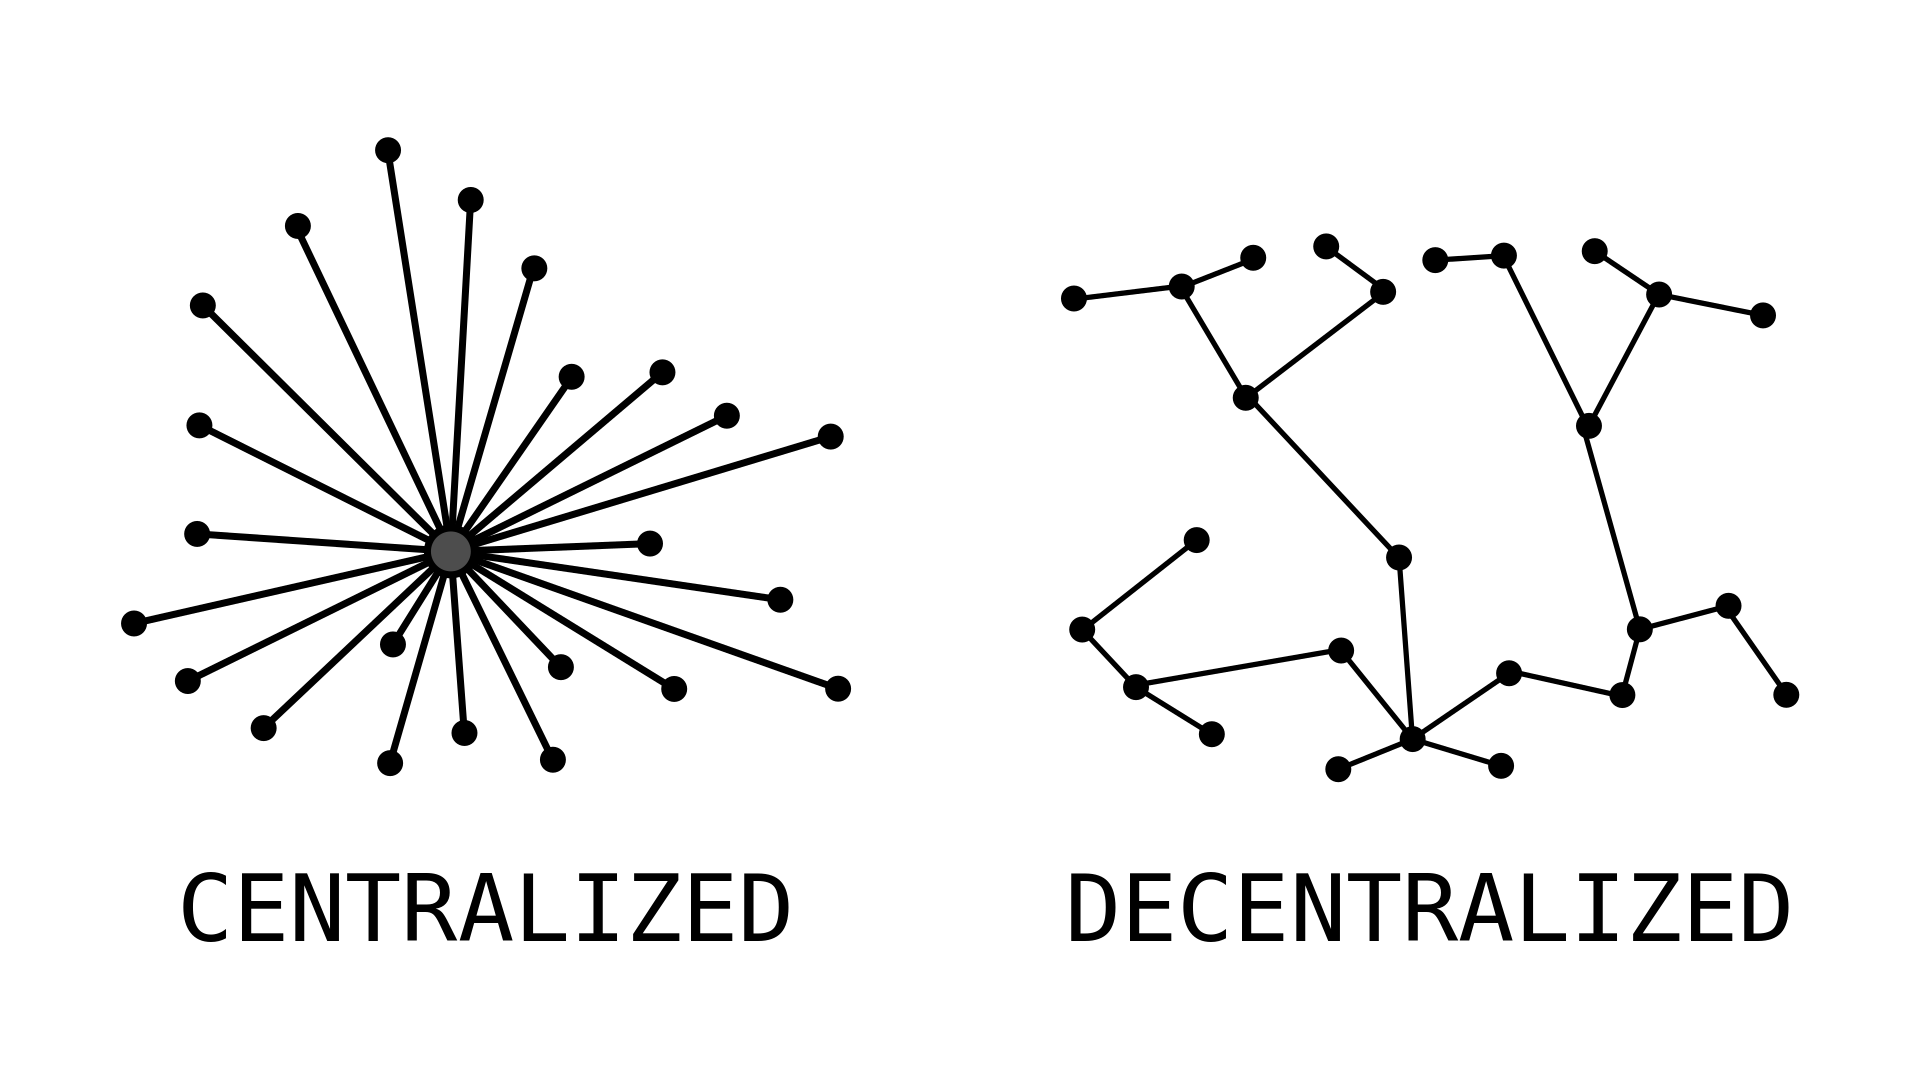
\includegraphics[width=0.7\textwidth]{Figures/Decentralization_diagram.png}
    \caption{Diagrama explicando la descentralización}
    \label{fg:decentralization_diagram}
    \cite{web:decentralization}
\end{figure}
Las criptomonedas, permiten liberarnos de los intermediarios: consiguen que las transacciones se realicen entre dos personas sin necesidad de transmitir esa información por multiples canales.
\subsection{Ethereum}
Ethereum es la evolución natural de Bitcoin. En su propio \textit{whitepaper}, hablan de cómo Bitcoin es un estado de transición, justificando que ethereum tiene más bloques de construcción para permitir crear un internet descentralizado. Ethereum aporta cambios sustanciales a la forma en la que es minado y crea un nuevo concepto llamado \textit{smart contracts}, que permite la ejecución automática de código en respuesta a eventos que ocurren en la red.
% TODO: citar
Todos los eventos, son tratados como mensajes. Es un término parecido a las “transacciones” clásicas en Bitcoin. Estos mensajes no son simplemente envíos de dinero, ya que pueden ser información enviada a \textit{smart contracts}. Una transacción, en ethereum tiene las siguientes partes:
\begin{center}
    \begin{table}[h!]
        \begin{tabular}{|p{0.3\linewidth} | p{0.58\linewidth}|}
            \hline
            Mensaje & Mensaje que quiere ser enviado \\
            \hline
            Firma   & Prueba criptográfica que verifica que el \textit{sender} es quien dice ser. \\
            \hline
            Atributos especiales & \\
            \hline
            STARTGAS &  Para evitar la ejecución de un bucle infinito en el minero, se impone un límite de gas que se va quemando mientras la ejecución avanza. Cuanto más se tarde en ejecutar más gas se quema. \\
            \hline
            GASPRICE & Por cada unidad de gas quemada, se le pagará al minero con su equivalencia en ether. \\
            \hline
        \end{tabular}
        \label{tab:ethereum_msg}
        \cite{web:transaction}
        \caption{Tabla explicando el desglose de un mensaje de ethereum.}
    \end{table}
\end{center}
Gracias a estos atributos especiales, podemos generar una experiencia de usuario mejor.
\begin{itemize}
    \item Si alguna transacción llegase a fallar, se le devolvería el gas restante. Estos fallos se pueden '\textit{elevar}' con \texttt{require}. Esta \textit{keyword} (palabra clave \cite{web:keyword}) reservada espera un '\textit{booleano}' con evaluación positiva.
Este código muestra \texttt{require} en funcionamiento.
\begin{lstlisting}
    function foo()
    public
    {
        // ... 
        // La ejecucion continua
        require(true,
        'Mensaje para enviar al sender si llega a fallar');
        // Si algun check llega a fallar se revierte el estado 
        require(false,
        'El sender vera este mensaje ya que el booleano es falso');
        // ...
    }
\end{lstlisting}
    \item Si alguna transacción se queda sin gas, el estado se revierte al inicial pero el dinero se pierde.
\end{itemize}

\subsection{Minería}
La minería es el proceso de verificar las transacciones que ocurren en la red. En el momento actual, el sistema de verificación que se utiliza es \textit{proof-of-work}. Al usar el mismo mecanismo de protección, sus transacciones se parecen.
\begin{figure}[h!]
    \centering
    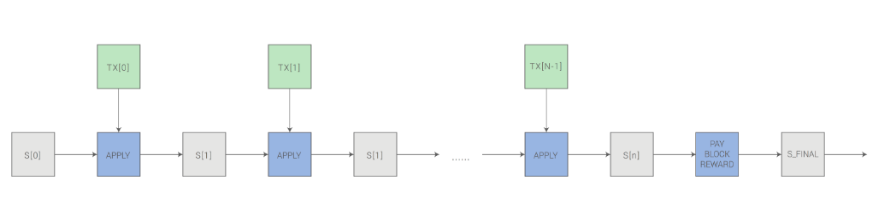
\includegraphics[width=0.8\textwidth]{Figures/Screenshot_20220507_131504.png}
    \caption{Diagrama que explica la mineria}
    \cite{web:block}
    \label{fg:block_diagram}
\end{figure}
La red de ethereum siempre se asegura que se genera un bloque cada 12 segundos.
Estos 12 segundos son una especie de latido que muestra la salud de la red de ethereum. Para mantener siempre ese ritmo, se ajusta la dificultad de minado. El proceso de minería sigue los siguientes pasos.
\begin{enumerate}
    \item Se genera una transacción y se firma con la clave privada.
    \item El usuario comparte la petición a toda la red de ethereum desde un minero.
    \item En algún momento de esos 12 segundos, un minero puede llegar a agregar cientos de transacciones en un posible bloque, en una manera que maximiza las comisiones de transacción. Todo esto mientras están por debajo del limite de gas.
    \begin{enumerate}
        \item Verifica la legitimidad de la transacción: Por ejemplo que la firma corresponde al mensaje y que la cuenta tenga liquidez.
        \item Inicia el proceso de \textit{proof of work}.\\ 
        Este proceso se basa en los siguientes parámetros. Dificultad del bloque ex:
        \texttt{3,324,092,183,262,715}, mixHash ex.\\ \texttt{0x44bca881b07a6a09f83b130798072441705d9a665c5ac8bdf2f39a3cdf3bee29} y la sal (número hexadecimal aleatorio) 
        \texttt{0xd3ee432b4fb3d26b}. \textit{Proof-of-work} es una carrera entre todos los mineros de la red para ver quien puede generar un \textit{hash} \cite{web:hash}. Cuando se genera un \textit{hash} con SHA 256 ex. \\
        \texttt{ba7816bf8f01cfea414140de5dae2223b00361a396177a9cb410ff61f20015ad} se busca que tenga que tenga una cierta cantidad de ceros al principio. La dificultad del bloque es cuántos \textit{hashes} pueden ser correctos para ese bloque. Cuanto menor sea el número, más difícil es verificar ese bloque.
    \end{enumerate}
    \item Eventualmente, algún minero conseguirá solucionar el puzzle criptográfico y nuestro mensaje estará aceptado en la \textit{blockchain}. Ese bloque contiene el \textit{checksum} (Suma de verificación \cite{web:checksum}) de todos los elementos internos.
    \item El resto de la red, al escuchar que un minero ha conseguido solucionar el bloque, lo verifica y si es correcto lo toma como el estado canónico de la red.
    \item Por ultimo los mineros borran de su memoria la lista de su \textit{mempool}. \cite{web:mining}
\end{enumerate}
\textbf{Limitaciones}\\
\textit{Proof-of-work}, como se ha explicado, es una operación computacionalmente intensa. En una red congestionada como está en estos momentos \cite{web:gas_price}, la dificultad de los bloques está explotada. Aún así, el consumo energético, comparando con otras \textit{blockchains} famosas, es inferior \ref{fg:consumo}. Esto hace que si tenemos aproximadamente 70 transacciones en un bloque, estamos gastando 5880000 Wh.
\begin{figure}[H]
    \centering
    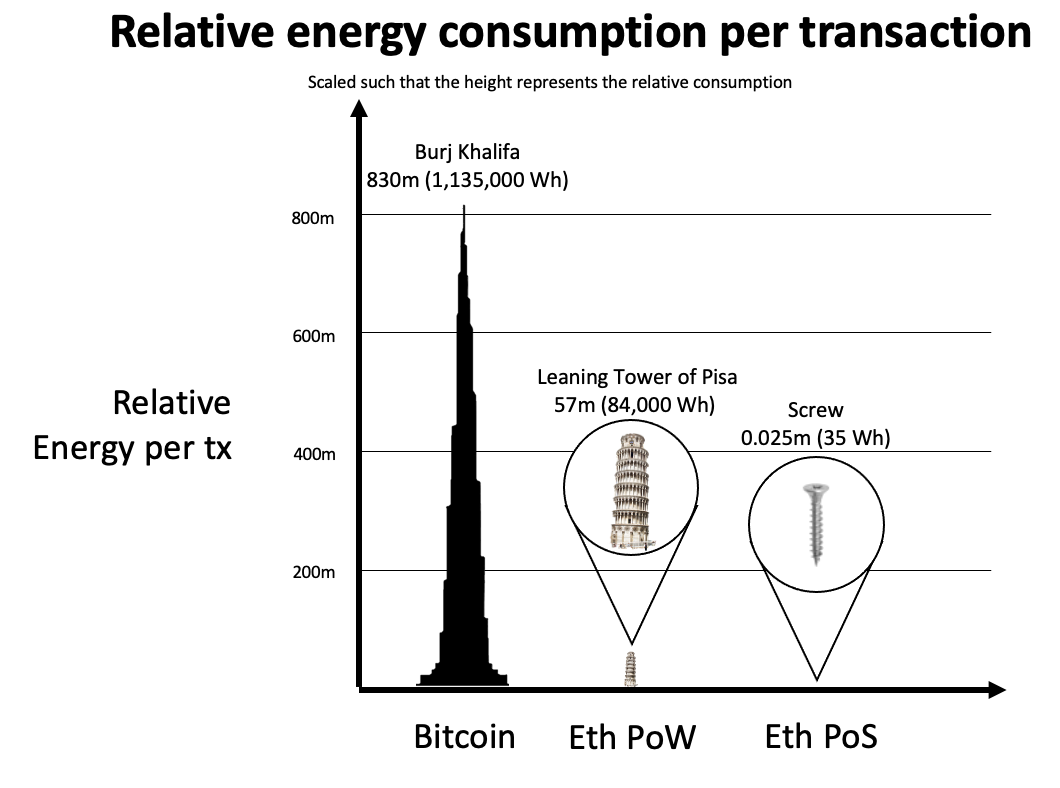
\includegraphics[width=0.6\textwidth]{Figures/consumo.png}
    \caption{Diagrama comparativo de consumo energético por transacción}
    \label{fg:consumo}
    \cite{web:eth_energy}
\end{figure}
Ethereum quiere actualizar su método de verificación a \textit{proof-of-stake}. Esto cambiaría a un modo de verificación computacionalmente caro a otro que no lo es tanto. Antes de que ese cambio ocurra, Ethereum seguirá consumiendo en un año lo mismo que Finlandia y tendrá una huella de carbono comparable a Bulgaria \cite{web:carbono}.
A fecha de publicación de este proyecto, Ethereum 2.0 no está implementado. Desde 2016 se lleva retrasando una bomba de dificultad para migrar a los usuarios, pero aún \textit{no ha explotado}. Esta bomba existe para evitar que se cree una copia. Esto hará que la dificultad crezca de manera exponencial hasta que minar un nuevo bloque sea imposible. Se lleva retrasando año tras año, hasta un total de 5 veces. Por ahora tiene fecha de junio de 2022. Aún así, en el EIP-4345 \cite{web:eip_bomb}, se da la posibilidad de retrasarlo aún más.
Hasta que no se haga el cambio de algoritmo de verificación, Ethereum seguirá contaminando. Esta implicación ética se investigará en el apartado correspondiente.
\subsection{Gas}
Como se ha explicado antes, se puede ejecutar código en la red de ethereum. Para proteger la red, existe una pequeña tarifa que hay que pagar por cada unidad de tiempo de ejecución. Así se evita la existencia de ataques por parte de actores malignos. Cuando una transacción se completa, se envía de vuelta el gas resultante al origen \ref{fg:message_diagram}.
\begin{figure}[h!]
    \centering
    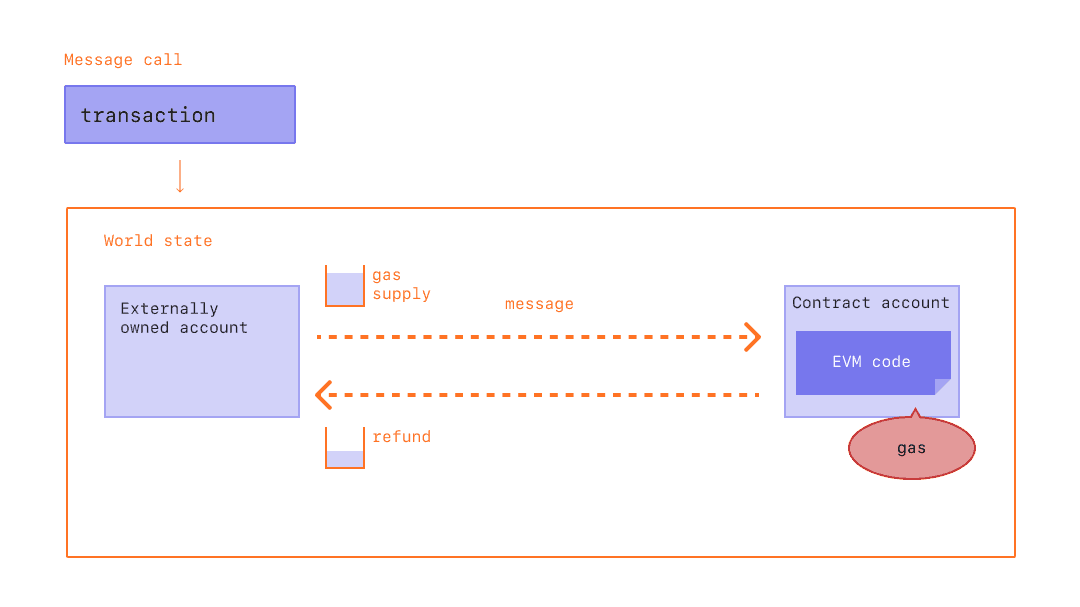
\includegraphics[width=0.8\textwidth]{Figures/gas-tx.png}
    \caption{Diagrama que explica el uso de gas}
    \label{fg:message_diagram}
\end{figure}
\begin{equation}
    max fee - (base fee + tip) = refund
\end{equation}
Después de la \textit{London update} \cite{web:london}, el gas en ethereum ha evolucionado para proteger más a los usuarios de posibles manipulaciones por parte de los mineros. Esta limitación se explicará más adelante.
\subsection{Smart Contracts}
Un \textit{smart contract} (Contrato inteligente \cite{web:scontract}) es un programa que vive en la \textit{blockchain}. A niveles prácticos, un contrato es como si fuese otra persona de la red con la que interactuamos.
Si nosotros tenemos la dirección
\begin{quote}
    \verb|0xc0ffee254729296a45a3885639AC7E10F9d54979|
\end{quote}
un contrato puede tener la dirección
\begin{quote}
    \verb|0x70E3Aed5aA1aac6EC39D114B7411DF6f1CC80671|
\end{quote}
Todos los mensajes compartidos entre los usuarios y un \textit{smart contract} quedan grabados para siempre en la cadena de bloques global. Como se ha dicho anteriormente, en Ethereum las transacciones se llaman mensajes, porque su contenido no es simplemente dinero, puede tener una infinidad de funciones.
\begin{lstlisting}
    pragma solidity 0.8.7;

    contract VendingMachine {
    
        // Declare state variables of the contract
        address public owner;
        mapping (address => uint) public cupcakeBalances;
    
        // When 'VendingMachine' contract is deployed:
        // 1. set the deploying address as the owner of the contract
        // 2. set the deployed smart contract's cupcake balance to 100
        constructor() {
            owner = msg.sender;
            cupcakeBalances[address(this)] = 100;
        }
    
        // Allow the owner to increase the smart contract's 
        // cupcake balance
        function refill(uint amount) public {
            require(msg.sender == owner, "Only the owner can refill.");
            cupcakeBalances[address(this)] += amount;
        }
    
        // Allow anyone to purchase cupcakes
        function purchase(uint amount) public payable {
            require(msg.value >= amount * 1 ether, 
            "You must pay at least 1 ETH per cupcake");
            require(cupcakeBalances[address(this)] >= amount,
            "Not enough cupcakes in stock to complete this purchase");
            cupcakeBalances[address(this)] -= amount;
            cupcakeBalances[msg.sender] += amount;
        }
    }
\end{lstlisting}
Tomando de ejemplo el código de la \textit{wiki} de Ethereum, se va a explicar su funcionamiento. \cite{web:sample_smart_contract}.
Solidity, el lenguaje de programación DSL (domain specific language \cite{web:DSL}) que utiliza la \textit{blockchain} Ethereum, tiene un paradigma de programación basado en objetos. Por eso mismo, su sintaxis es similar a los lenguajes \textit{C-like}, por ejemplo java.
En el siguiente bloque de código, especificamos la version de solidity que vamos a utilizar; En este caso y a fecha de publicación de este proyecto es la siguiente: \verb|0.8.7|.
\begin{lstlisting}
    pragma solidity 0.8.7;
\end{lstlisting}
Después podemos definir nuestro objeto. Para este ejemplo, vamos a crear una maquina de \textit{vending}.
\begin{lstlisting}
    contract VendingMachine {//...}
\end{lstlisting}
En este lugar, funcionaría de una manera parecida a un programa clásico en java. Las variables de ese objeto se pueden declarar directamente, estableciendo si son públicas o privadas. Ser pública significaría que esa variable es accesible por otros objetos, permitiendo utilizar su valor o modificarlo directamente. Ser privada, significa que solo puede ser usada por el objeto que la crea.
En nuestra máquina dispensadora, se va  a guardar la dirección del creador para poder por ejemplo reponer la maquina. Solidity tiene un tipo nativo que puede guardar direcciones directamente.
\begin{lstlisting}
    address public owner;
\end{lstlisting}
Ahora solo se necesita llenar la maquina. En este punto, podemos crear un mapa que asocie cantidades a direcciones concretas.
Si la dirección de nuestro contrato es \verb|0x70...0671| podemos hacer que si buscamos el valor asociado a esa dirección obtengamos el balance.
\begin{lstlisting}
    mapping (address => uint) public cupcakeBalances;
\end{lstlisting}
Para poder llenar la máquina nada más instalarla, existe el constructor. Un método constructor en java se ejecuta cuando se crea una nueva instancia del objeto con la \textit{keyword} \verb|new|. En este caso, nuestro constructor es llamado una vez se añade a la \textit{blockchain}. Por este motivo, nos cuesta gas hacer \textit{deploy} (despliegue) de un contrato.
\begin{lstlisting}
    // When 'VendingMachine' contract is deployed:
    // 1. set the deploying address as the owner of the contract
    // 2. set the deployed smart contract's cupcake balance to 100
    constructor() {
        owner = msg.sender;
        cupcakeBalances[address(this)] = 100;
    }
\end{lstlisting}
Por último, tenemos las funciones clásicas. En una maquina solo se puede añadir elementos y que alguien los compre. Estas funciones se pueden crear con la \textit{keyword} \verb|function|. Pueden comportarse como \textit{voids} o como una persona a la que pagar con \verb|payable|.
Gracias a \verb|require|, podemos crear puntos de control, que por ejemplo permitan que solo el creador pueda añadir más magdalenas a la máquina. No solo eso, sino que podemos asegurarnos que tengan el dinero necesario y que queden magdalenas en la máquina.
\begin{lstlisting}
    // Allow the owner to increase the smart contract's cupcake balance
    function refill(uint amount) public {
        require(msg.sender == owner, "Only the owner can refill.");
        cupcakeBalances[address(this)] += amount;
    }

    // Allow anyone to purchase cupcakes
    function purchase(uint amount) public payable {
        require(msg.value >= amount * 1 ether, 
        "You must pay at least 1 ETH per cupcake");
        require(cupcakeBalances[address(this)] >= amount, 
        "Not enough cupcakes in stock to complete this purchase");
        cupcakeBalances[address(this)] -= amount;
        cupcakeBalances[msg.sender] += amount;
    }
\end{lstlisting}
\textbf{Limitaciones}\\
La gran limitación de los \textit{smart contracts} es la inmutabilidad de la red. Una vez se publica ese contrato, no se puede actualizar. Si se descubre un fallo o se quiere cambiar la lógica se necesita volver a publicar el contrato. Esto implica que no solo el contrato sigue existiendo para siempre, sino que hay que direccionar a nuestros usuarios al nuevo contrato.
Como se explicará mas adelante, esto supone que hay que cambiar la dirección que le aportamos a los usuarios a través de nuestro \textit{payload} de js.
\subsection{Puntos débiles de la solución elegida}
Antes de la \textit{London Update} \cite{web:london}, los mineros podían llegar a manipular el precio ralentizando la ejecución y usando todo el gas del usuario. Esto suponía que los usuarios que quisieran hacer una transacción, se encontraban con la necesidad de llenar con más gas su transacción para que algún minero la ejecutase en un tiempo aceptable. El resto de usuarios, si querían que su transacción no tardase 30 minutos como mínimo, tendría que inevitablemente pagar más.
Para evitar eso, se introdujo un límite de gas en cada bloque. Ademas, los usuarios podían poner un rango de gas que estarían dispuestos a pagar. De esta forma, se busca que los bloques sean lo mas eficientes posibles.
Actualmente, tanto la dificultad de los bloques como el gas medio de transacción está disparado\cite{web:gas_price}. Esto hace que cualquier transacción tenga un coste añadido. Moderadores de r/ethereum dicen lo siguiente cuando son preguntados sobre si el alto precio del gas ``\textit{matará} '' a Ethereum:
\begin{displayquote}
    \textbf{High gas fees will kill Ethereum}\\
    This is one of those bizarre comments that pervades through crypto retail doesn't seem to make any sense. Overwhelming demand for a product will somehow... kill a project? It's like saying AMD and Nvidia are going to die soon because graphics cards are now grotesquely overpriced.
    No, the reality, like I said above, is that there's overwhelming demand for EVM blockspace and a limited supply of gas. Currently, the high fees shows there's incredible demand for Ethereum L1 blockspace, and people are willing to pay a steep premium for it.
    This is what gives the Ethereum network and ETH value. And in two months' time, there'll be a mechanism with EIP-1559 to accrue this value to every ETH stakeholder.
    Over time, we will see gas fees drop with a greater supply of gas - the reality is that there'll never quite be enough blockspace supply to satisfy global demand for EVM blockspace long term. There'll be rollups, there'll be hybrid solutions like zkPorter/Validium, there'll be sidechains/alternate chains, and there'll be centralized solutions. The ecosystem will work together to offer different trade-offs with decentralization versus transaction fees.
    \cite{web:reddit_ethereum}
\end{displayquote}
Aunque queda mucha discusión en los comentarios.
\begin{displayquote}
    Your answer for fees is far from being satisfying. Yes high fees will kill Eth. Your Nvidia example isn't the same thing.
    You know there are other successful blockchains coming strong. Avalanche for one has lots of Dapps on it. People will quit using Eth at some point if this doesn't change. Because other chains have already solved that problem...
    And I wouldn't care about any supply problem for a global demand, because this won't be an issue. We all use Eth because we have to and we all know it.
    \cite{web:reddit_ethereum_comment}
\end{displayquote}
Es un problema que los contribuidores de Ethereum tendrán que combatir y probar en una de la redes más grandes del mundo. Como Ethereum es código abierto, se pueden crear \textit{Ethereum Improvement Proposals} - EIP \cite{web:EIP}. De esta manera la comunidad puede mejorar y actualizar la red.
\section{Introducción a envíos de datos a través de un medio distribuido}
\begin{displayquote}
    IPFS is a distributed system for storing and accessing files, websites, applications, and data. \cite{web:ipfs_whatis}
\end{displayquote}
IPFS \cite{web:ipfs} es una red descentralizada que permite compartir datos de manera muy sencilla. IPFS consigue tener una mayor distribución del ancho de banda.
Todos los nodos de la red pueden estar conectados entre si teniendo una interconexión eficiente. Los ficheros subidos a IPFS tienen un CID (Content IDentifier). Ese CID es un registro permanente de la existencia de ese fichero como existe en el tiempo.
Cuando otro usuario busca tu CID \ref{fg:looking_for_CID}, pregunta al resto de los usuarios dónde esta el fichero. Cuando lo reciben, lo \textit{cachean} y se convierten en proveedores de tu fichero.
\begin{figure}[H]
    \centering
    
\includegraphics[width=0.2\textwidth]{Figures/svgviewer-png-output.png}
    \caption{Diagrama que explica la búsqueda de un CID}
    \label{fg:looking_for_CID}
    \cite{web:ipfs}
\end{figure}
Un usuario, puede anclar (pin) un fichero para guardar y proveerlo para siempre. En cambio, los contenidos que no tengan ese \textit{pin} serán descartados para liberar memoria. Los usuarios solo guardan lo que les interesa, más un pequeño índice para saber lo que tienen otros usuarios.
Todos los ficheros van acompañados de un \textit{checksum}; Si alguien intenta cambiar el fichero o sus datos, provocará un cambio en el \textit{hash}. Esto implica que se le asignará un CID distinto. Nuestros ficheros una vez subidos están seguros y serán resistentes ante la censura y la manipulación \ref{fg:keeping_IPFS_safe}.
En la siguiente sucesión de figuras, ponemos a prueba los pasos para iniciar una conexión.
\begin{center}
\begin{figure}[h!]
    \centering
    
\includegraphics[width=0.2\textwidth]{Figures/svgviewer-png-output(2).png}
    \caption{Diagrama que explica la protección ante censura}
    \label{fg:keeping_IPFS_safe}
    \cite{web:ipfs}
\end{figure}
\end{center}
\subsection{Servidores Star}
Para que los nodos se puedan encontrar, primero necesitan contactar con algún nodo conocido.
Para que eso ocurra, se tienen las siguientes opciones.
\begin{enumerate}
    \item Tablas de \textit{hashing} distribuidas.
    \item Paquetes \textit{broadcast} en la red local.
    \item Compartir listas de \textit{peers} con \textit{peers} conocidos.
    \item \textit{Trackers} o puntos de encuentro centralizados.
    \item Lista de servidores Star
\end{enumerate}
Los servidores son muy útiles ya que te devuelven información de dónde están tus \textit{peers} más cercanos con los que poder empezar a compartir.
Para comprender mejor la situación, vamos a ver unas figuras.
\begin{itemize}
    \item Tenemos un servidor Star que tiene metadatos de los \textit{peers} que están cerca.
    \item Las líneas grises son conexiones pasadas que han dejado el rastro del \textit{handshake} (saludo).
    \item Las líneas negras son conexiones activas de IPFS (libp2p).
    \item La figura verde quiere entrar a la red.
\end{itemize}
\begin{figure}[h!]
    \centering
    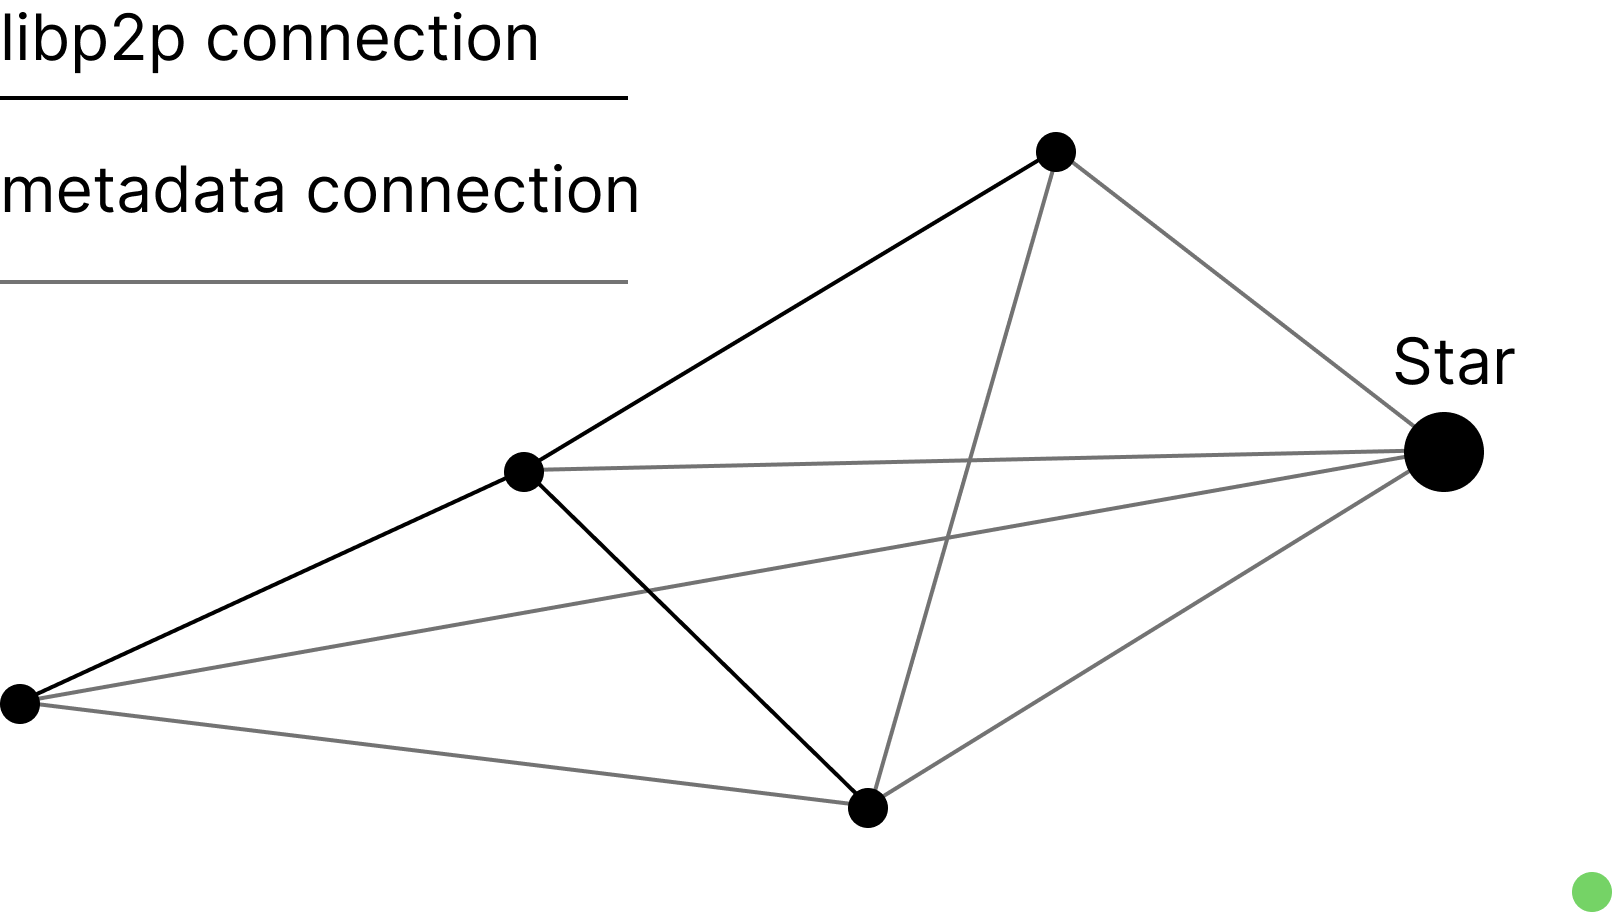
\includegraphics[width=0.7\textwidth]{Figures/Green wants to join(2).png}
    \caption{Diagrama en el que el nodo verde quiere entrar en la red IPFS}
    \label{fg:scanning_ipfs}
\end{figure}
\begin{figure}[h!]
    \centering
    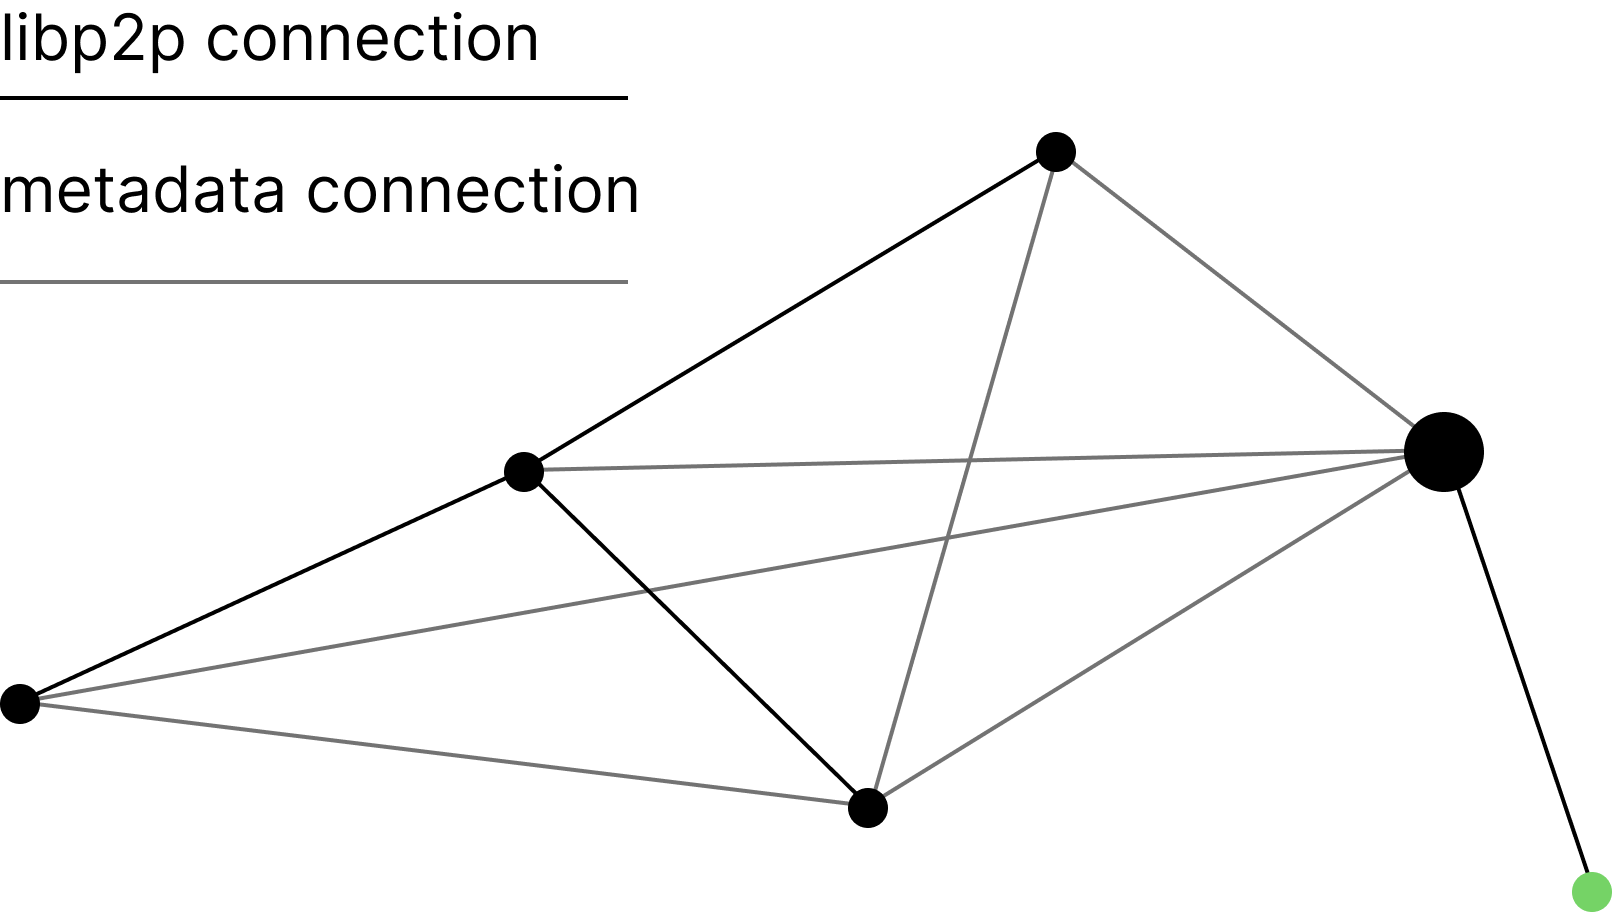
\includegraphics[width=0.7\textwidth]{Figures/Green ask Star for instructions.png}
    \caption{Diagrama en el que el nodo verde pregunta a Star dónde están el resto de las personas}
    \label{fg:asking_star}
\end{figure}
\begin{figure}[h!]
    \centering
    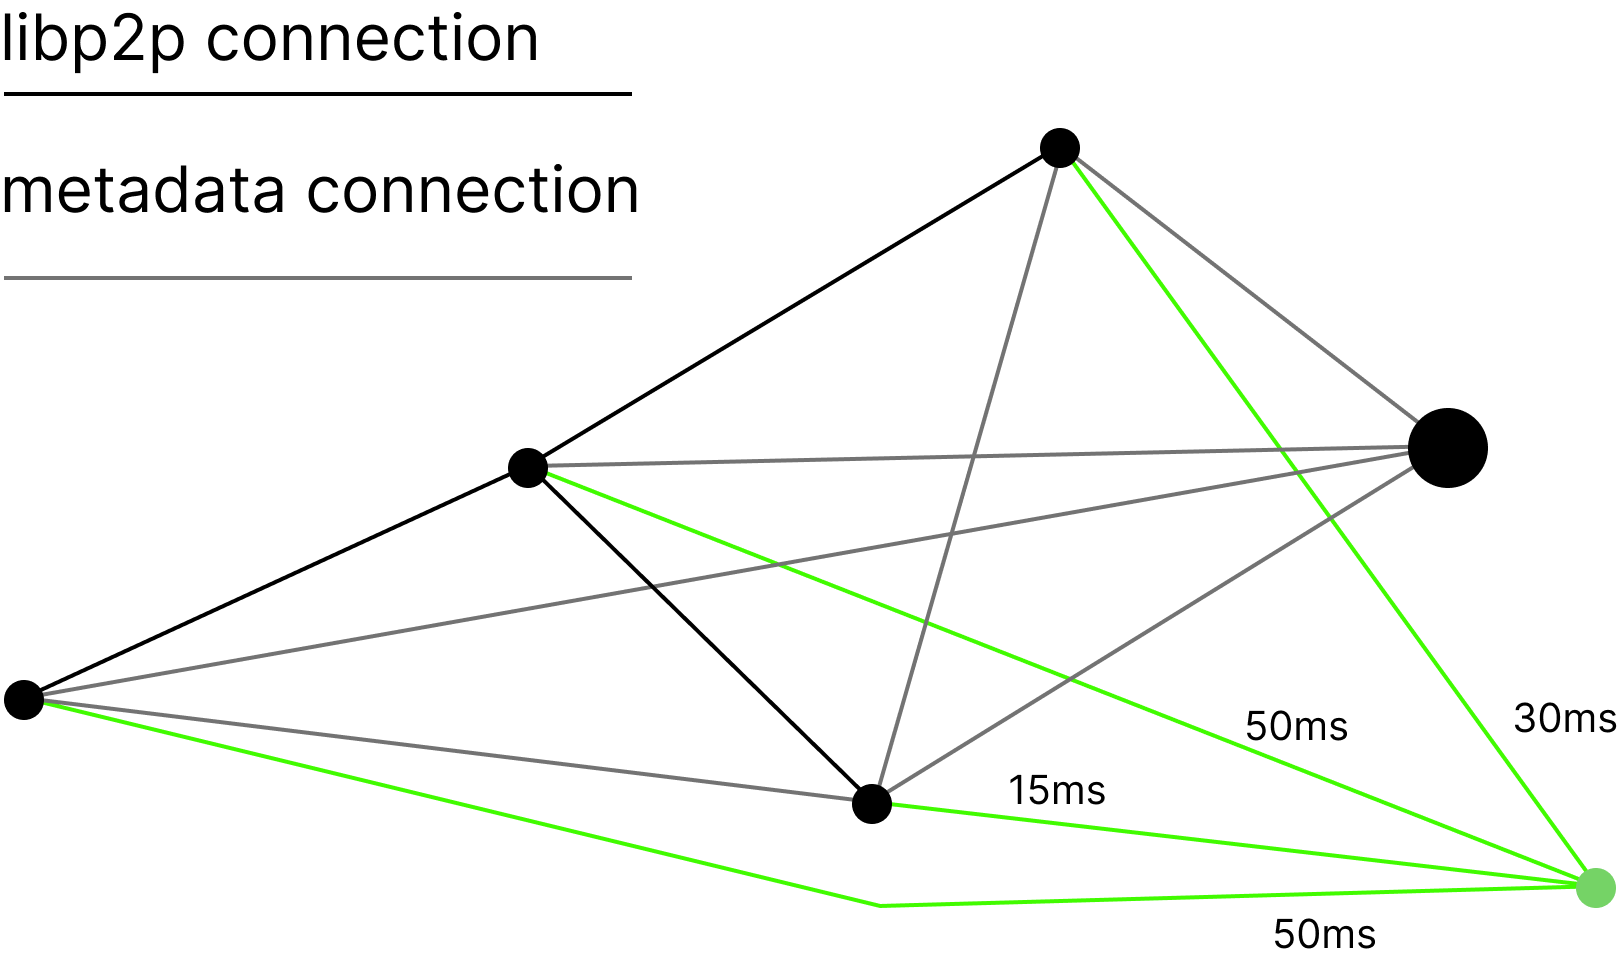
\includegraphics[width=0.7\textwidth]{Figures/Green scans the other peers.png}
    \caption{Diagrama en el que el nodo verde escanea sus alrededores para ver qué conexión es más eficiente}
    \label{fg:scanning_area}
\end{figure}
\begin{figure}[h!]
    \centering
    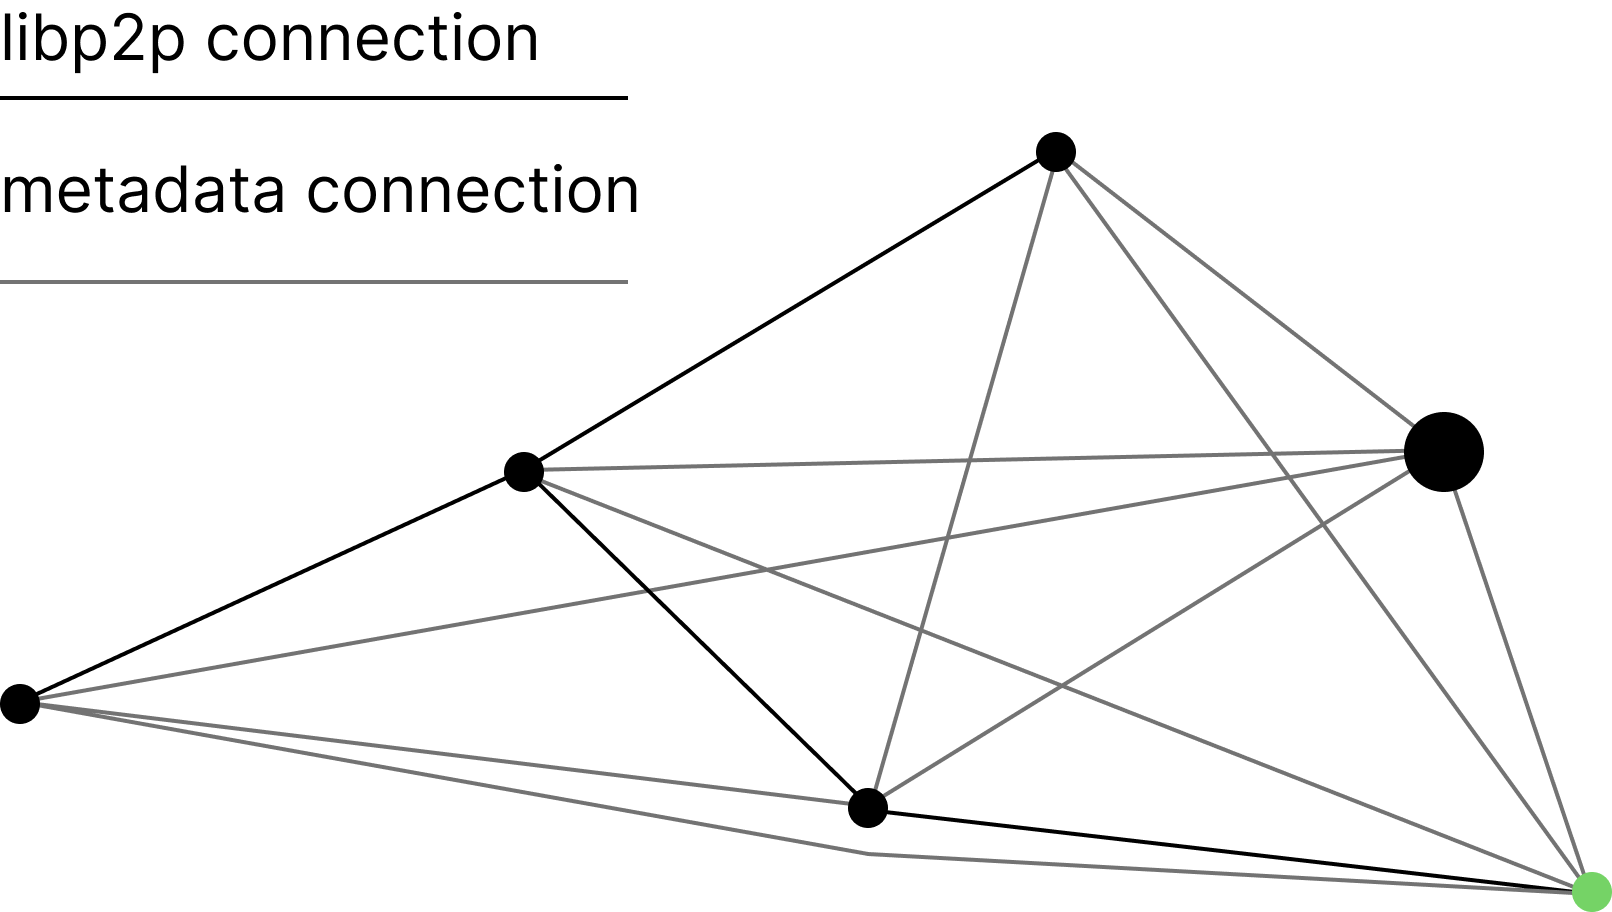
\includegraphics[width=0.7\textwidth]{Figures/Green finally joins(1).png}
    \caption{Diagrama en el que el nodo verde finalmente se conecta}
    \label{fg:connecting}
\end{figure}
\subsection{Nodos y relés}
Los nodos son los usuarios a los que se hacía referencia anteriormente. Estos nodos pueden ser: usuarios verídicos ejecutando \verb|js-ipfs| \cite{web:js-ipfs} en su navegador, o una instancia de \verb|go-ipfs| \cite{web:go-ipfs} o \verb|js-ipfs| en un servidor para garantizar nodos de alta velocidad.
Estos nodos tienen un repositorio en el que guardan fragmentos de datos que están alojando o bien que han pasado por él y ha cacheado.
Otra función principal de un nodo es retransmitir información. Para realizar esta función, tienen que estar conectados a otros nodos de la manera que hemos visto en el punto anterior.
\begin{figure}[H]
    \centering
    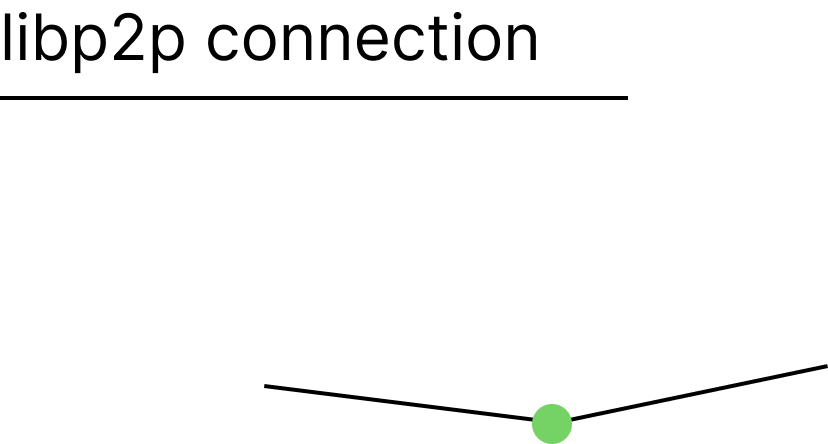
\includegraphics[width=0.4\textwidth]{Figures/Angulo 2.png}
    \caption{El nodo de color verde tiene un nivel de red 2. Ya que hay dos conexiones activas.}
    \label{fg:network_dgr}
\end{figure}
Primero vamos a ver el concepto de nivel de red. Las opciones predeterminadas de libp2p para el nivel ideal es \verb|6|. Un nivel entre \verb|4| - \verb|12| es un nivel \textit{aceptable}.
\begin{quote}
    Por simplicidad en los diagramas el \textit{Lower bound} (nivel inferior) = 2 y el \textit{Upper bound} (nivel superior) = 4.
\end{quote}
Viendo esto, necesitamos un modo inteligente en el que asegurar que todos los nodos reciben la información sin duplicidades.
\begin{figure}[h!]
        \centering
        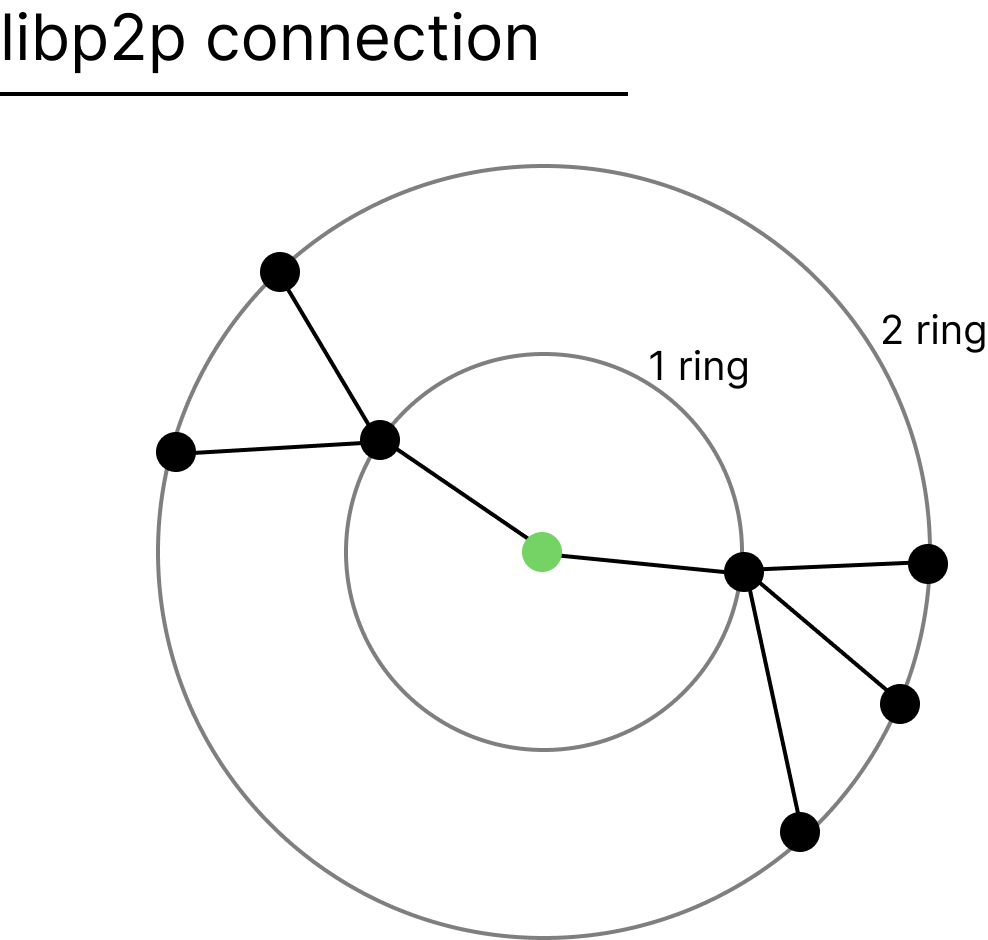
\includegraphics[width=0.5\textwidth]{Figures/Radios de comunicacion.png}
        \caption{Mapa de conexiones desde el punto de vista del nodo verde. \textbf{La conexión de metadatos ha sido omitida por razones de claridad.}}
        \label{fg:Mapa_de_conexiones}
\end{figure}
En la figura \ref{fg:Mapa_de_conexiones}, si un dato del ring 2 quiere llegar hasta el nodo verde, aparentemente, al no tener una conexión directa no podría hacerlo, pero como los nodos actúan de \textit{relays}, los datos pueden pasar por el ring 1 hasta llegar al nodo verde.
Al hacerlo, los nodos que viven en el ring 1, si los datos han pasado por ellos, pueden guardar esos datos para que si el nodo verde los vuelve a solicitar, se le envíen con menor latencia.
Aplicando \textit{pruning} (poda), el grafo anterior quedaría de la siguiente manera \ref{fg:mapa_optimizado}.
\begin{figure}[H]
    \centering
    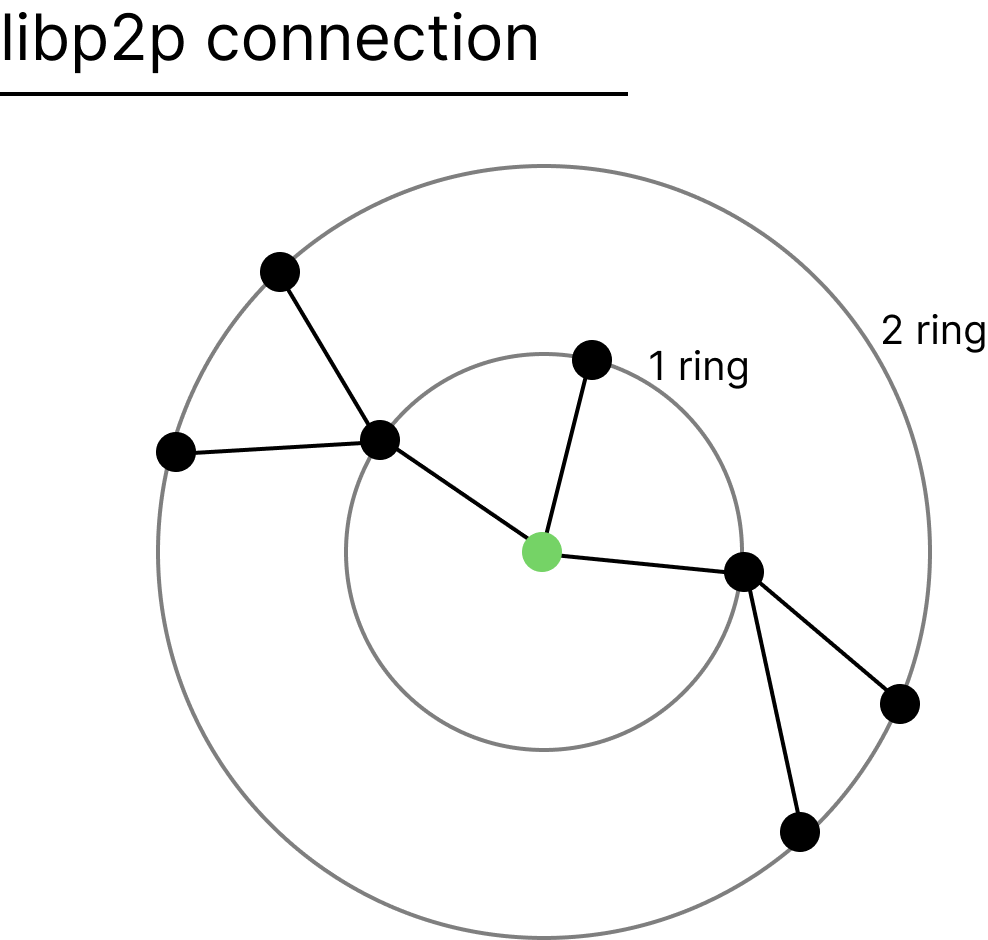
\includegraphics[width=0.5\textwidth]{Figures/Radios de comunicacion optimizado.png}
    \caption[El nodo verde optimiza la conexión]{El nodo verde optimiza la conexión. \textbf{El nodo movido, también calcularía cual seria su conexión óptima, pero todas las conexiones se ven desde el punto de vista del nodo verde.}}
    \label{fg:mapa_optimizado}
\end{figure}
Esto significa que como el nivel de conexión óptimo es 3, en la figura original \ref{fg:Mapa_de_conexiones} la red no es óptima. Nuestro nodo verde tiene 2 y el nodo en la parte inferior derecha tiene 4. Para poder generar un grafo más óptimo, el nodo verde tendría que tener 3 conexiones y el nodo en la parte inferior derecha también. Por eso mismo nuestro nodo verde inicia una nueva conexión óptima y el nodo en la parte inferior derecha borra una conexión, resultando en \ref{fg:mapa_optimizado}.
\subsection{PubSub}
PubSub \ref{fg:PubSub}, es una parte del \textit{spec} (especificación) de IPFS, fundamental para el funcionamiento del proyecto.
PubSub, permite subscribirse a un topic. Un \textit{topic} se define con un \verb|string|.
Pongamos como ejemplo que existen los siguientes topics.
\begin{figure}[h!]
    \centering
    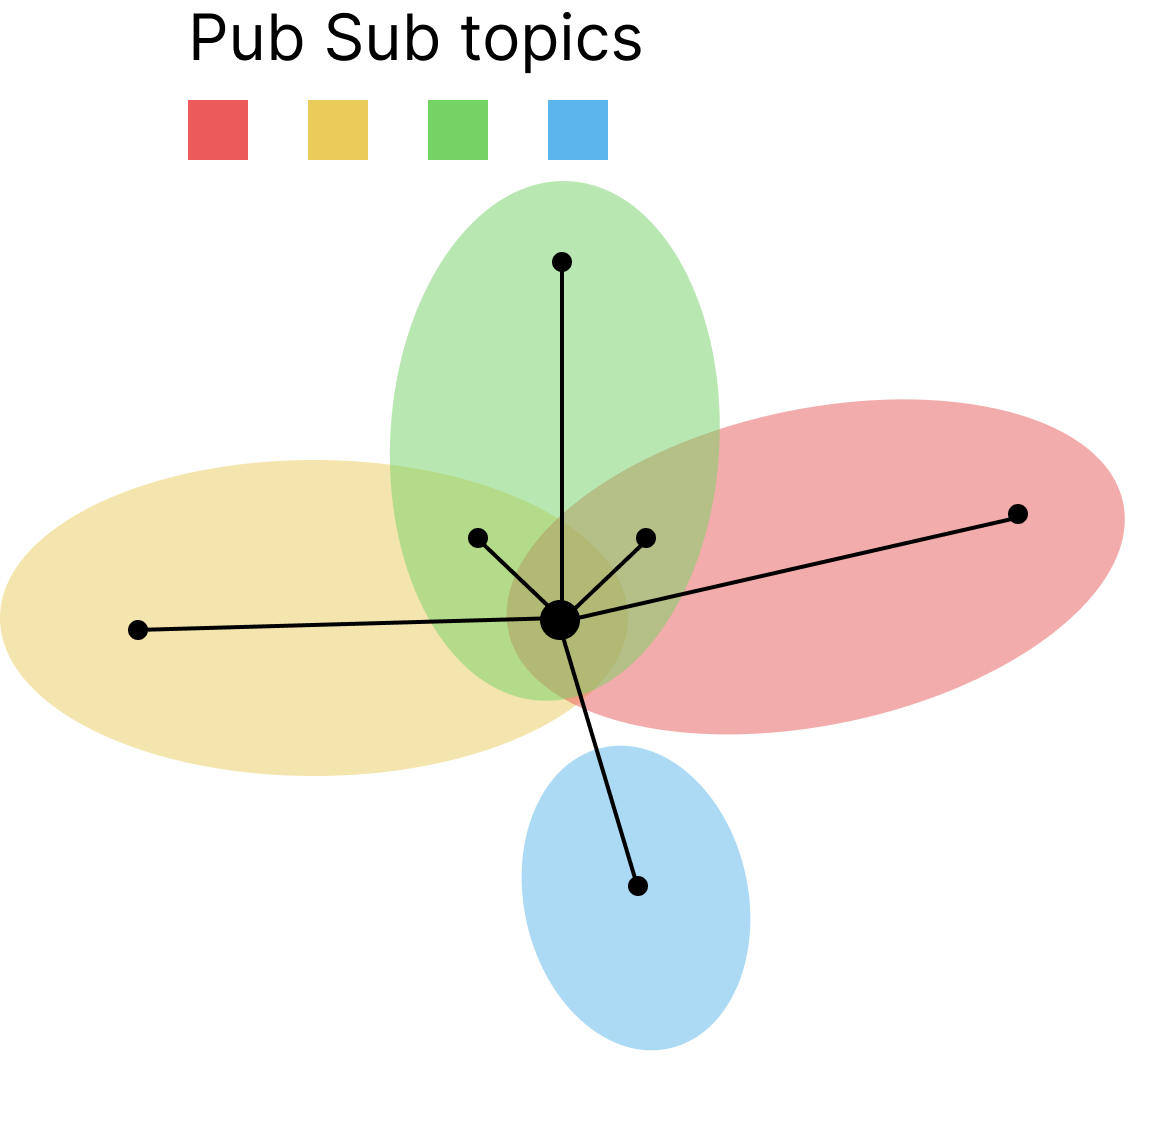
\includegraphics[width=0.7\textwidth]{Figures/Pub Sub.png}
    \caption{Diagrama explicando el funcionamiento de PubSub. Punto de vista del nodo central.}
    \label{fg:PubSub}
\end{figure}
\begin{itemize}
    \item \verb|Rojo|
    \item \verb|Verde|
    \item \verb|Amarillo|
    \item \verb|Azul|
\end{itemize}
El \textit{host} central, está subscrito a los \textit{topics} \verb|Amarillo|, \verb|Verde| y \verb|Rojo|.  Aun así, el nodo central está conectado a un nodo solo subscrito a un \textit{topic} \verb|Azul|. Esto se debe a que \verb|libp2p| intentará mantener una conexión saludable. Nuestro nodo no está solo interesado en escuchar a su \textit{topic}, sino ayudar a establecer una red saludable en la que hacer llegar la información necesaria a todos los nodos interesados.
\begin{figure}[H]
    \centering
    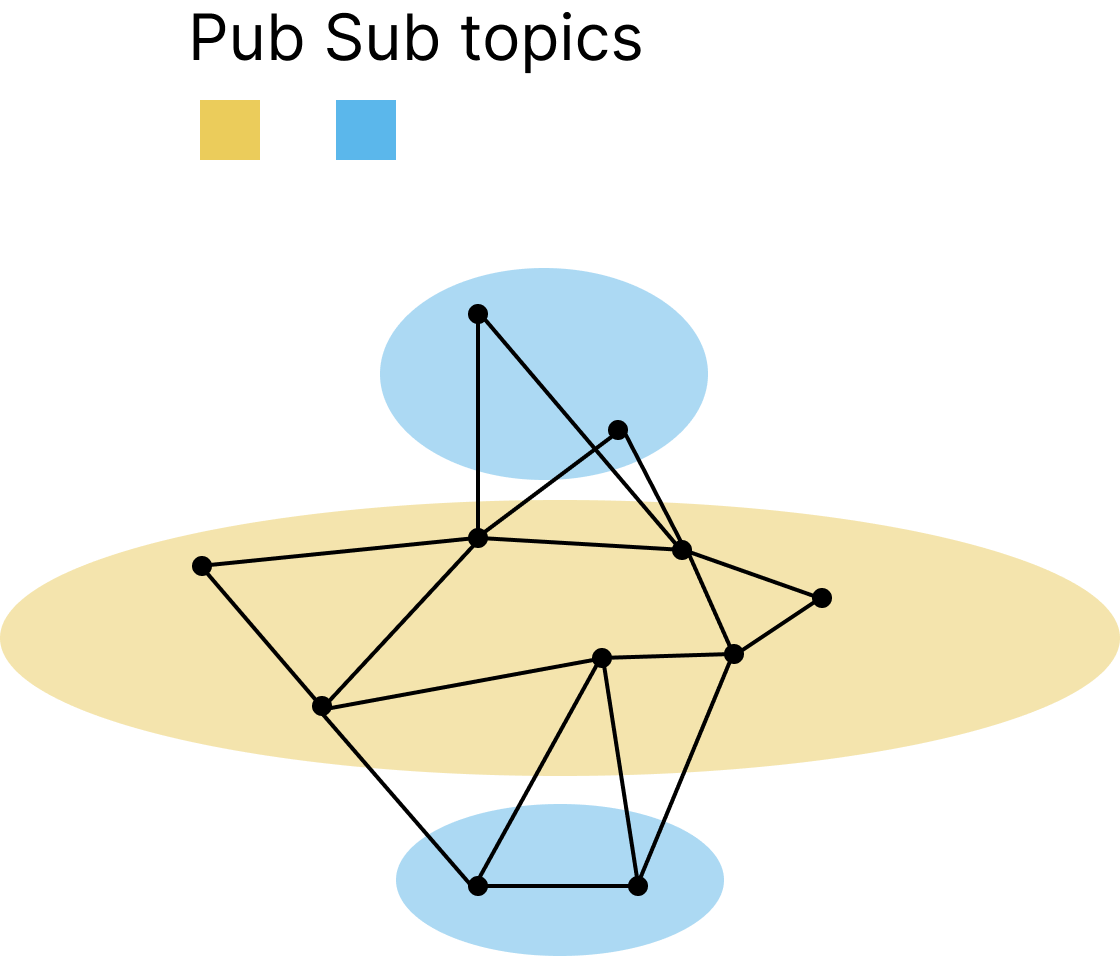
\includegraphics[width=0.7\textwidth]{Figures/Zonas multiples.png}
    \caption{Grafo de ejemplo para explicar la donación de temas.}
    \label{fg:zonas_multiples}
\end{figure}
En este posible grafo de conexión \ref{fg:zonas_multiples}, hay 4 hosts que están subscritos al tema \verb|Azul|. Si los \textit{host} que están escuchando al \textit{topic} \verb|Amarillo| no pasasen el mensaje, las dos zonas azules no estarían comunicadas.
Los nodos comparten todos los mensajes y guardan metadatos de los mensajes que pasar por ellos. Por eso, los nodos que escuchan al \textit{topic} amarillo, pueden hacer de relés y pasar todos los mensajes.
De este modo, IPFS nos permite crear una red global de envío de mensajes instantáneos de manera gratuita y con un sistema resistente a fallos, ya que nuestros paquetes tienen varias rutas por las que ir y reparten carga entre las rutas posibles.
\subsection{Alternativas}
A la hora de compartir información de manera distribuida, hay muchas opciones. Una de ellas, también muy popular en el presente, es webtorrent \cite{web:webtorrent}: Un librería que trae las tecnologías Torrent a la web.
Este proyecto, utiliza \verb|webrtc| lo mismo que IPFS para conseguir la funcionalidad. \verb|Webrtc| no se usa en el resto de la red. Significando que existe una brecha en la misma. Aunque los dos se basen en un archivo \verb|.torrent|, si no tienes \textit{peers} compartiendo esa información utilizando un cliente compatible, no puedes acceder a él.
\begin{figure}[H]
    \centering
    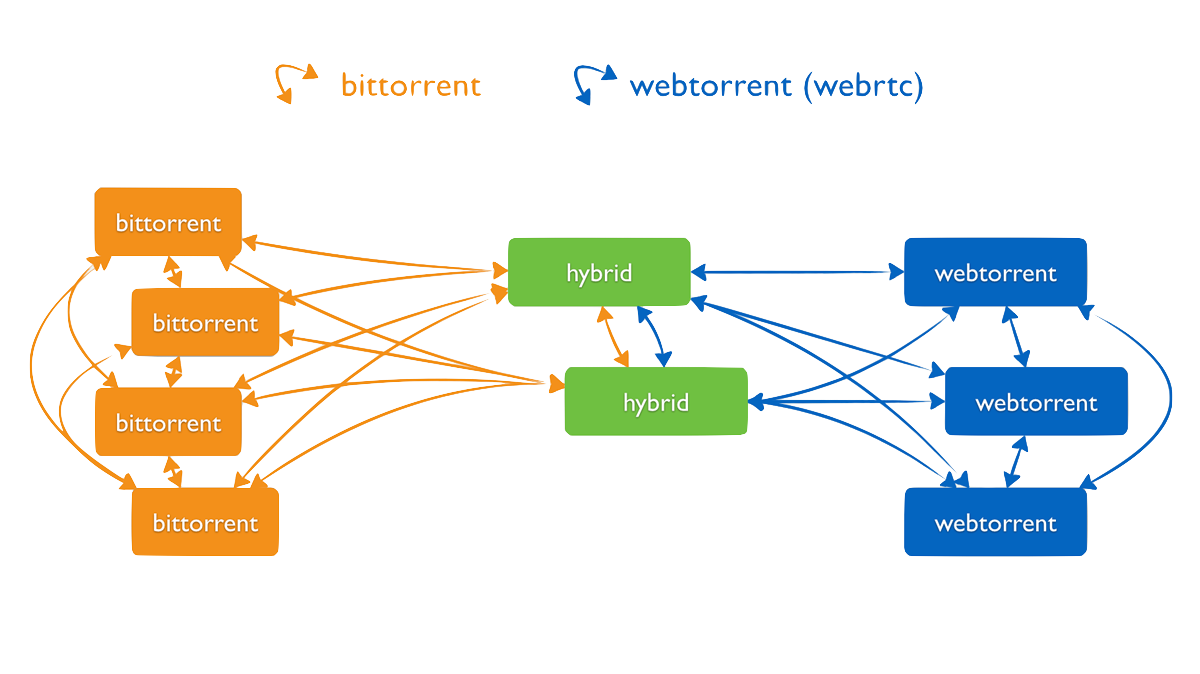
\includegraphics[width=0.6\textwidth]{Figures/68747470733a2f2f776562746f7272656e742e696f2f696d672f6e6574776f726b2e706e67.png}
    \caption{Diagrama explicando la división en la red de bit/web-torrent.}
    \cite{web:torrent}
    \label{fg:webtorrent}
\end{figure}
En la web, dan las herramientas a desarrolladores de programas \verb|torrent| a implementar un adaptador entre las dos redes. Por ahora solo \textbf{WebTorrent Desktop, Vuze, webtorrent-hybrid, Playback, instant.io y \(\beta\)Torrent} han implementado un adaptador, convirtiéndose en un nodo \textbf{\textit{hybrid}}.\\
% TODO: Explorar wormhole %
\textbf{Desventajas de utilizar WebTorrent}\\
Como ya se ha comentado hay una division en la red. Las tecnologías p2p se benefician de tener una gran cantidad de nodos. En cambio en este proyecto al haber una division, no se puede llegar a potencial teórico.
Otra gran desventaja es la \textbf{inmutabilidad}.
\begin{quote}
    \textbf{Is it possible to do live streaming with WebTorrent?}\\
    WebTorrent cannot do live streaming out-of-the-box, however you can build a live streaming solution on top of WebTorrent.
    Torrents are immutable. That means that once a torrent file is created, it cannot be changed without changing the info hash. So, how could one get around this limitation?
    A naive approach would be this: The content producer could take every 10 seconds of live content and create a torrent for it. Viewers would follow this \textit{feed} of torrent files (or info hashes) and download the content sequentially. Streamers would be around 10-20 seconds behind the live stream.
    This approach can definitely be improved, thougH Why not give that a shot yourself and share the code? \cite{web:webtorrent_faq}
\end{quote}
IPFS, aunque también sea inmutable por naturaleza para protegerse de censura y manipulación, implementa PubSub, una manera de poder propagar cambios en la red. 
Esto hace que en el archivo que reside en el DID solo exista el \textit{topic} y la identidad de esa persona. Como la base de datos es solo de esa persona, solo ella misma la que puede añadir identidades o retirarlas. Eso hace que las personas que estén escuchando al \textit{topic} de IPFS también puedan comprobarlo.
\newpage
\section{Introducción a la criptografía}
Este trabajo requiere criptografía para poder garantizar la seguridad de los datos compartidos. Como hemos visto, los datos compartidos en IPFS, por cualquier nodo que pasan, son cacheados para permitir una baja latencia en futuros accesos. Esto es un problema, ya que de manera predeterminada IPFS no incorpora encriptación de contenido.
\begin{quote}
    \textbf{IPFS docs}
    As a protocol for peer-to-peer data storage and delivery, IPFS is a public network: Nodes participating in the network store data affiliated with globally consistent content addresses (CIDs) and advertise that they have those CIDs available for other nodes to use through publicly viewable distributed hash tables (DHTs). This paradigm is one of IPFS's core strengths — at its most basic, it's essentially a globally distributed ``server'' of the network's total available data, referenceable both by the content itself (those CIDs) and by the participants (the nodes) who have or want the content.
    What this does mean, however, is that IPFS itself isn't explicitly protecting knowledge about CIDs and the nodes that provide or retrieve them. This isn't something unique to the distributed web; on both the d-web and the legacy web, traffic and other metadata can be monitored in ways that can infer a lot about a network and its users. Some key details on this are outlined below, but in short: While IPFS traffic between nodes is encrypted, the metadata those nodes publish to the DHT is public. Nodes announce a variety of information essential to the DHT's function — including their unique node identifiers (PeerIDs) and the CIDs of data that they're providing — and because of this, information about which nodes are retrieving and/or reproviding which CIDs is publicly available.
    So, why doesn't the IPFS protocol itself explicitly have a privacy layer built-in? This is in line with key principles of the protocol's highly modular design — after all, different uses of IPFS over its lifetime may call for different approaches to privacy. Explicitly implementing an approach to privacy within the IPFS core could "box in" future builders due to a lack of modularity, flexibility, and future-proofing. On the other hand, freeing those building on IPFS to use the best privacy approach for the situation at hand ensures IPFS is useful to as many as possible.\cite{web:ipfs_modularity}
\end{quote}
Hay dos tipos de encriptado:
\begin{itemize}
    \item Encriptado de transporte
    \item Encriptado de contenido
\end{itemize}
\subsection{Transporte}
La encriptación en el transporte \ref{fg:trasnporte} es usada cuando dos nodos quieren compartir información.
\begin{center}
    \begin{figure}[h!]
        \centering
        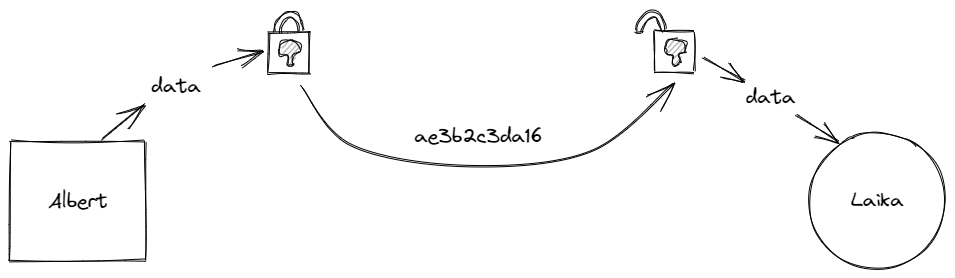
\includegraphics[width=0.7\textwidth]{Figures/transport-encryption.033b6a51.png}
        \caption{En esta figura, tenemos dos peers, que quieren enviar una información. IPFS encripta directamente la información haciendo imposible ver los datos \textbf{cuando están viajando de nodo en nodo}.}
        \label{fg:trasnporte}
        \cite{web:bias}
    \end{figure}
\end{center}
\subsection{Contenido}
La encriptación de contenido \ref{fg:contenido} se utiliza cuando se quiere asegurar que solo alguien que tiene la contraseña, pueda acceder al contenido.
\begin{center}
    \begin{figure}[h!]
        \centering
        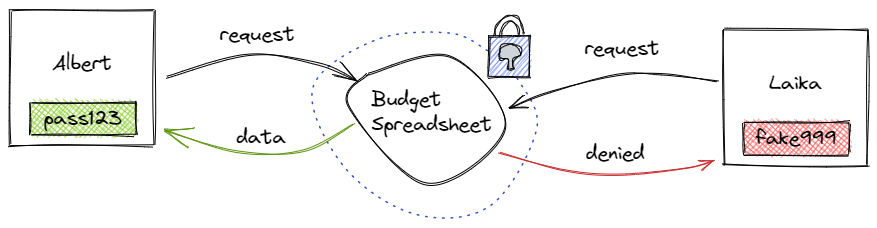
\includegraphics[width=0.7\textwidth]{Figures/content-encryption.adc5de58.png}
        \caption{En la figura, sin la contraseña correcta, Laika no puede acceder al fichero.}
        \label{fg:contenido}
        \cite{web:bias}
    \end{figure}
\end{center}
IPFS usa encriptación de transporte \ref{fg:trasnporte}, pero no encriptación de contenido \ref{fg:contenido}. Esto, según su \textit{wiki}, se hace para que no exista un \textit{bias} (sesgo de orientación \cite{web:bias}) a la hora de elegir qué tipo de encriptación es mejor para cada proyecto. Para este en concreto, se ha seleccionado una combinación de criptografía asimétrica con criptografía simétrica.
\subsection{XSalsa20 - Criptografía asimétrica}
La \textbf{criptografía asimétrica} (en inglés asymmetric key cryptography), \textbf{criptografía de clave pública} (en inglés public key cryptography) o \textbf{criptografía de dos claves} (en inglés two-key cryptography), es un sistema para poder compartir información utilizando claves públicas y privadas. Las claves públicas, como su nombre indica, son accesibles por todo el mundo. En cambio, la clave privada, tiene que permanecer protegida \cite{web:asimetrica}.
\begin{figure}[h!]
    \centering
    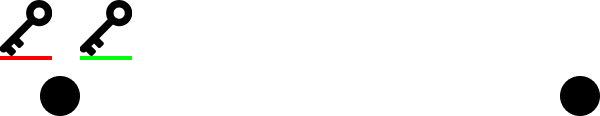
\includegraphics[width=0.7\textwidth]{Figures/Claves.png}
    \caption{Clave publica señalada en verde y la clave privada en rojo.}
    \label{fg:clave}
\end{figure}
Cuando el nodo de la derecha quiere enviar información a la que solo va a tener acceso el nodo de la izquierda, tiene que usar su clave pública \ref{fg:clave}.
\begin{figure}[h!]
    \centering
    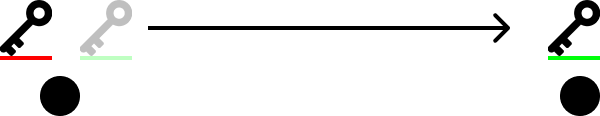
\includegraphics[width=0.7\textwidth]{Figures/Claves en movimiento(1).png}
    \caption{El host de la izquierda comparte su clave pública con el host de la derecha}
    \label{fg:movimiento}
\end{figure}
El nodo de la derecha, introducirá el mensaje en una caja y cerrará el candado utilizando esa llave. Ese candado solo puede ser abierto por la clave privada perteneciente al par original \ref{fg:movimiento}.
\begin{figure}[h!]
    \centering
    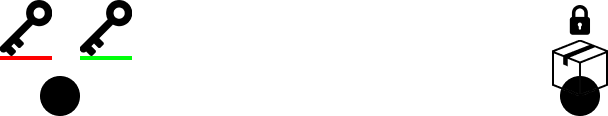
\includegraphics[width=0.7\textwidth]{Figures/Caja.png}
    \caption{El host de la derecha crea una \textit{caja}}
\end{figure}
Por último, lo único que queda es enviar esa caja a su destinatario; Esto se puede realizar por IPFS de manera segura.
NaCl pronunciada como ``sal'' es la librería de referencia, pero TweetNaCl \cite{web:tweetnacl}, consigue reducir el tamaño de NaCl, haciéndolo igual de rápido pero logrando que su código fuente quepa en 100 \textit{tweets}. De ahí su nombre.
\begin{quote}
    \textbf{Matthew D. Green, 2012}\\
    OpenSSL is the space shuttle of crypto libraries. It will get you to space, provided you have a team of people to push the ten thousand buttons required to do so. NaCl is more like an elevator—you just press a button and it takes you there. No frills or options.\\
    I like elevators. \cite{web:tweetnacl_elevator}
\end{quote}
\subsection{AES - Criptografía simétrica}
Aunque en teoría todas las comunicaciones se podrían hacer a través de criptografía asimétrica, para poder encriptar y desencriptar, se necesitan las claves de la cartera del usuario, estando limitados por el tamaño máximo que puedan soportar. Tenemos que comunicarnos con su cartera ya que nunca hay que dar la clave privada a nadie. Las claves privadas son propias y \textbf{siempre} deben serlo.
La criptografía simétrica se basa en una clave única. Cualquier entrada se puede encriptar y desencriptar con la misma clave. Para eso, a la hora de crear la caja para el usuario, generamos una contraseña aleatoria utilizando la \verb|api crypto| del navegador.
\begin{lstlisting}
    window.crypto.randomUUID()
\end{lstlisting}
\begin{quote}
    9fc2a1d0-5345-464c-a81e-a57a06b67669
\end{quote}
Después de esto se sigue el siguiente flujo.
\begin{itemize}
    \item Se encripta el fichero utilizando las \verb|apis| nativas de los navegadores.
    \item Anunciamos la existencia de un nuevo fichero en nuestro nodo de IPFS.
    \item En la caja introducimos el CID del fichero y la contraseña encriptada con la clave pública.
    \item Por último anunciamos por PubSub que se ha subido un fichero y que el destinatario puede abrirlo.
\end{itemize}
Para esta parte del proyecto se ha elegido AES ya que es muy popular, está soportado y tiene un buen historial de seguridad.
\newpage
\thispagestyle{empty}
\chapter{Objetivos y Alcance}\label{oya}
%Función que crea el título de capítulo y al cual se le da el nombre deseado a través de su parámetro obligatorio. Al no tener la función el “*” se escribirá también en el título del documento las palabras “Capítulo 1: …”. Además se indica, mediante la función “\label”, la correspondiente etiqueta que lleva asociada. La etiqueta sirve para que en caso de que luego se quiera hacer referencia al capítulo se haga llamando etiqueta tal que se escribiría “La información correspondiente a dicho tema se encuentra en el capítulo \ref{Int}.”

\thispagestyle{fancy}
%Función que determina que durante este capítulo se aplique el estilo Fancy.

\fancyhead[LE]{\thechapter.Objetivos y Alcance}


\section*{SSI}
SSI (Self sovereign identity) en ingles, es un un concepto en el la propia persona por existir, se representa a si mismo en internet. Esto, quiere decir que en internet nos dejaríamos de identificar utilizando correos electrónicos y pasaríamos a identificarnos por nuestra propia voluntad y una unión de clave publica y clave privada.

\section*{Introducción a las blockchain}
La blockchain, es un elemento importante para este proyecto. Su implementación, permite una comunicación segura y anónima entre personas, sin necesidad de ser verificada por terceros. Las blockchain, vienen en muchas formas y tipos, algunas siendo descentralizadas. Las mas populares, funcionan de manera puramente descentralizada, usando un sistema de prueba de trabajo para verificar todas las transacciones.

\newpage
\thispagestyle{empty}
%Funciones para incluir los otros documentos que se han desarrollado. Dichos documentos son los distintos capítulos de la memoria. Toda la escritura de los mismos se realizará en los documentos de forma específica y no en este archivo “MAIN.tex”. Así que vamos a ellos.

\bibliographystyle{unsrt}
%Función que indica el estilo de bibliografía a utilizar.
\bibliography{References.bib}
%Función que incluye la biblografía en el documento.

\end{document}